%\documentclass{article}
%\usepackage[utf8]{inputenc}

\documentclass[12pt]{article}
\usepackage{graphicx} % This lets you include figures
\usepackage{hyperref} % This lets you make links to web locations
\graphicspath{ {./images/} }

\usepackage[rightcaption]{sidecap}
\usepackage{subcaption}
\usepackage{wrapfig}

\usepackage{float}

\usepackage{imakeidx}
\usepackage{url}
\makeindex


\title{ARDF Automation Manual}
\author{}
\date{\today}

\begin{document}
\maketitle{}

\tableofcontents

\clearpage
\newpage






\section{Starting the ARDF Acquistion and Analysis Program}

%\maketitle{Setup}

\subsection{Click on Start Button and find the Spyder icon}

\begin{figure}[H]
 
    \begin{subfigure}{1\textwidth}
    
\includegraphics[scale=0.5]{images/spyder_icon.png} 
    \label{fig:DJp1}
    \end{subfigure}
%    \begin{subfigure}{0.5\textwidth}
%    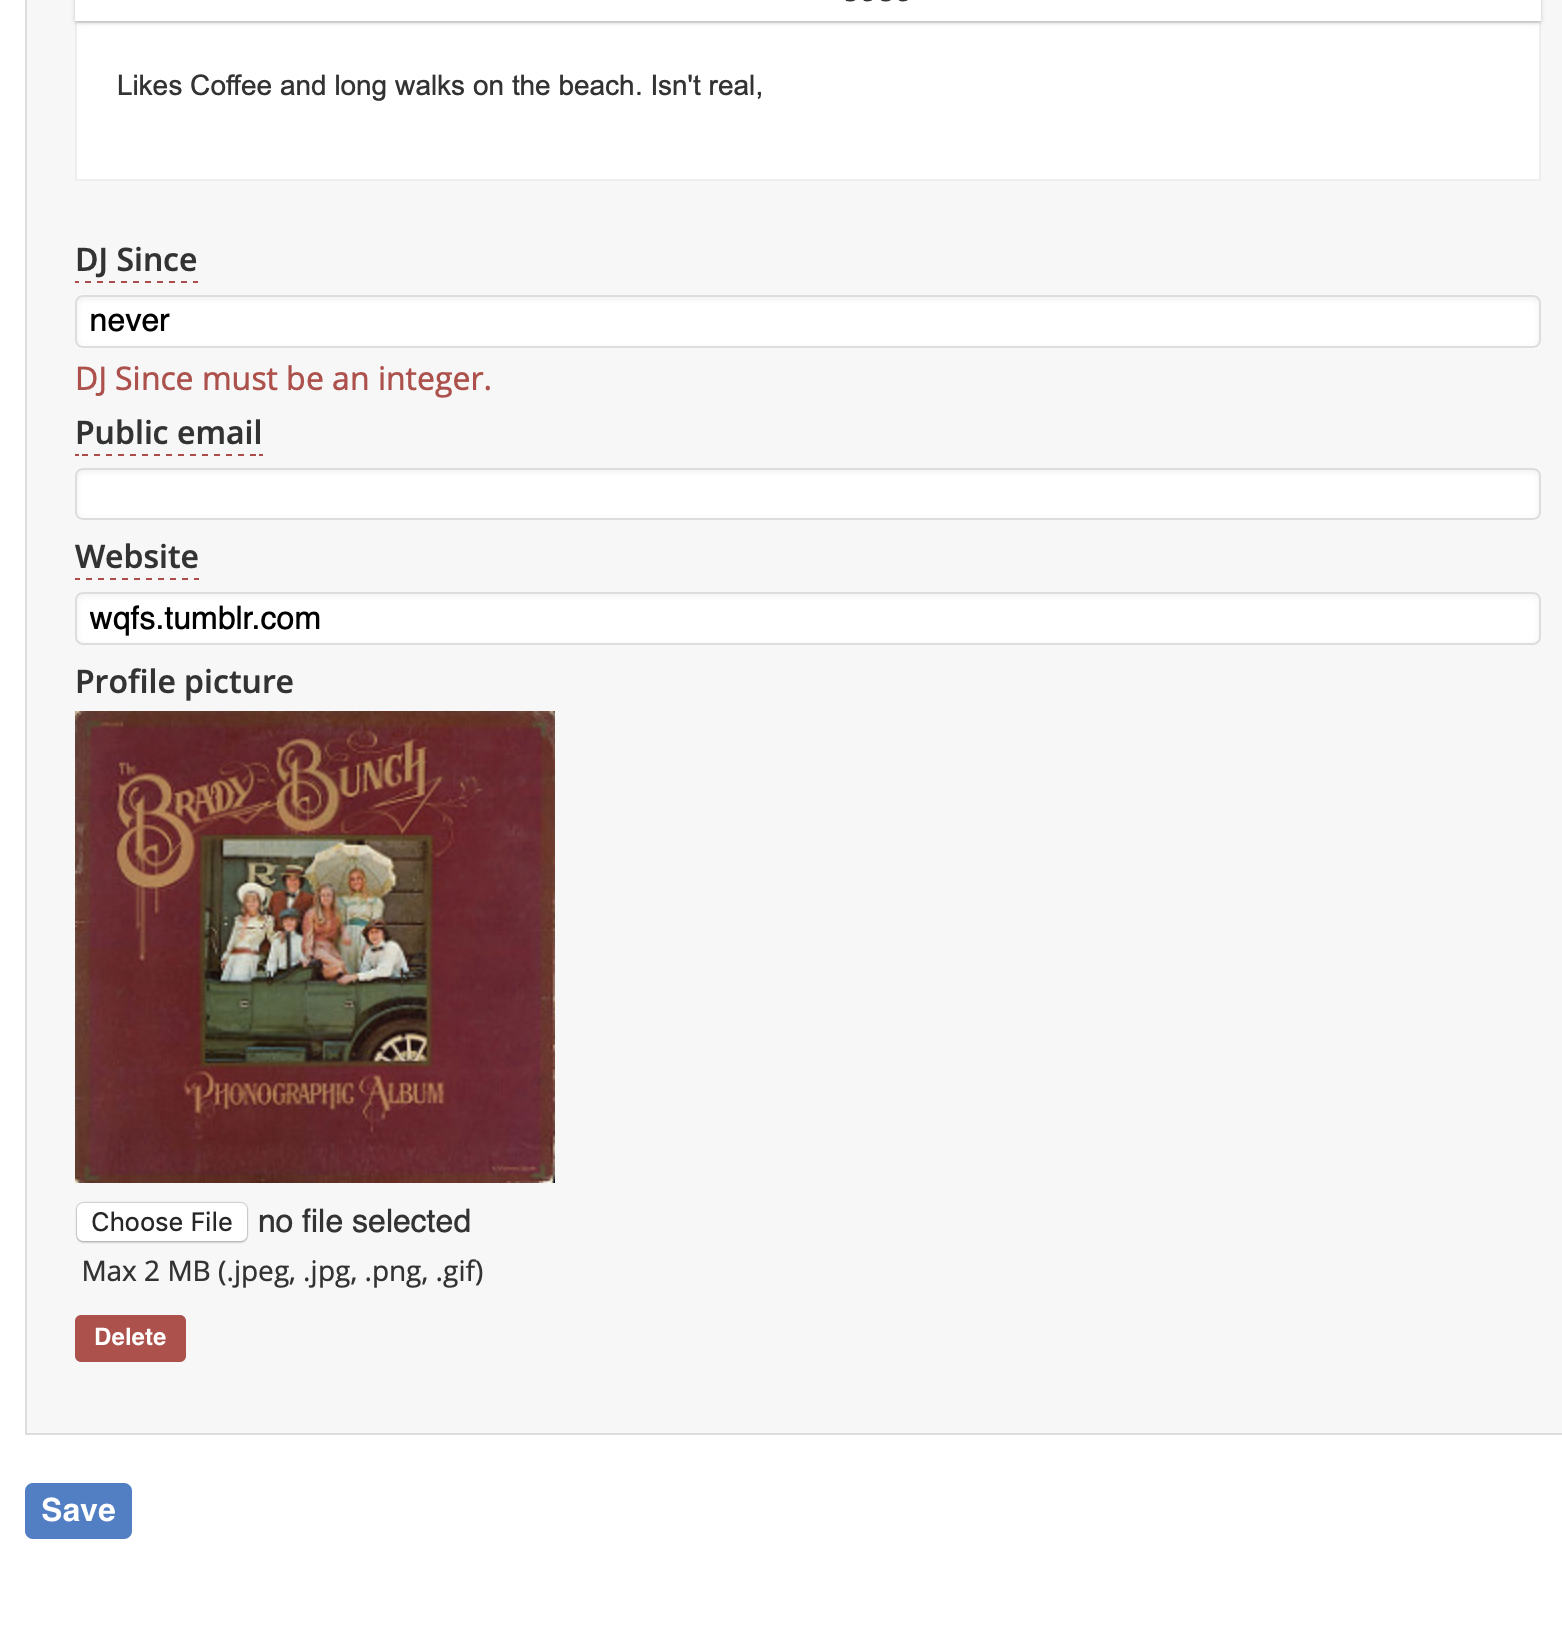
\includegraphics[width=1.0\linewidth, height=5cm]{images/DJ_profile2.png}
%    \label{fig:DJp2}
%    \end{subfigure}
 \caption{Spyder Icon to be found in the start menu}
\label{fig6}
\end{figure}




\subsection{Right Click and Run as Administrator }
These Administrator privileges are required for communicating with the RS 232 port, which is the protocol for connecting with the Agilent switch

\begin{figure}[H]
 
    \begin{subfigure}{1\textwidth}
    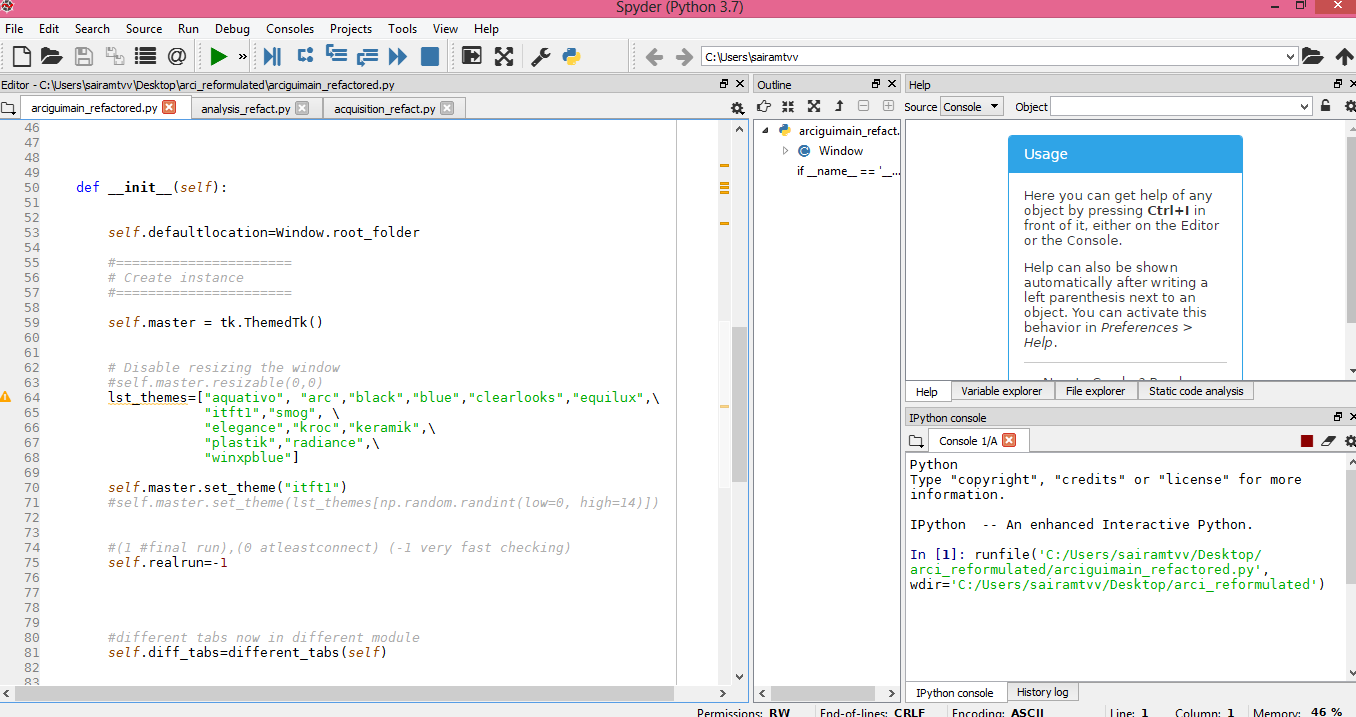
\includegraphics[scale=0.3]{images/spyder_console.png} 
    \label{fig:DJp1}
    \end{subfigure}
%    \begin{subfigure}{0.5\textwidth}
%    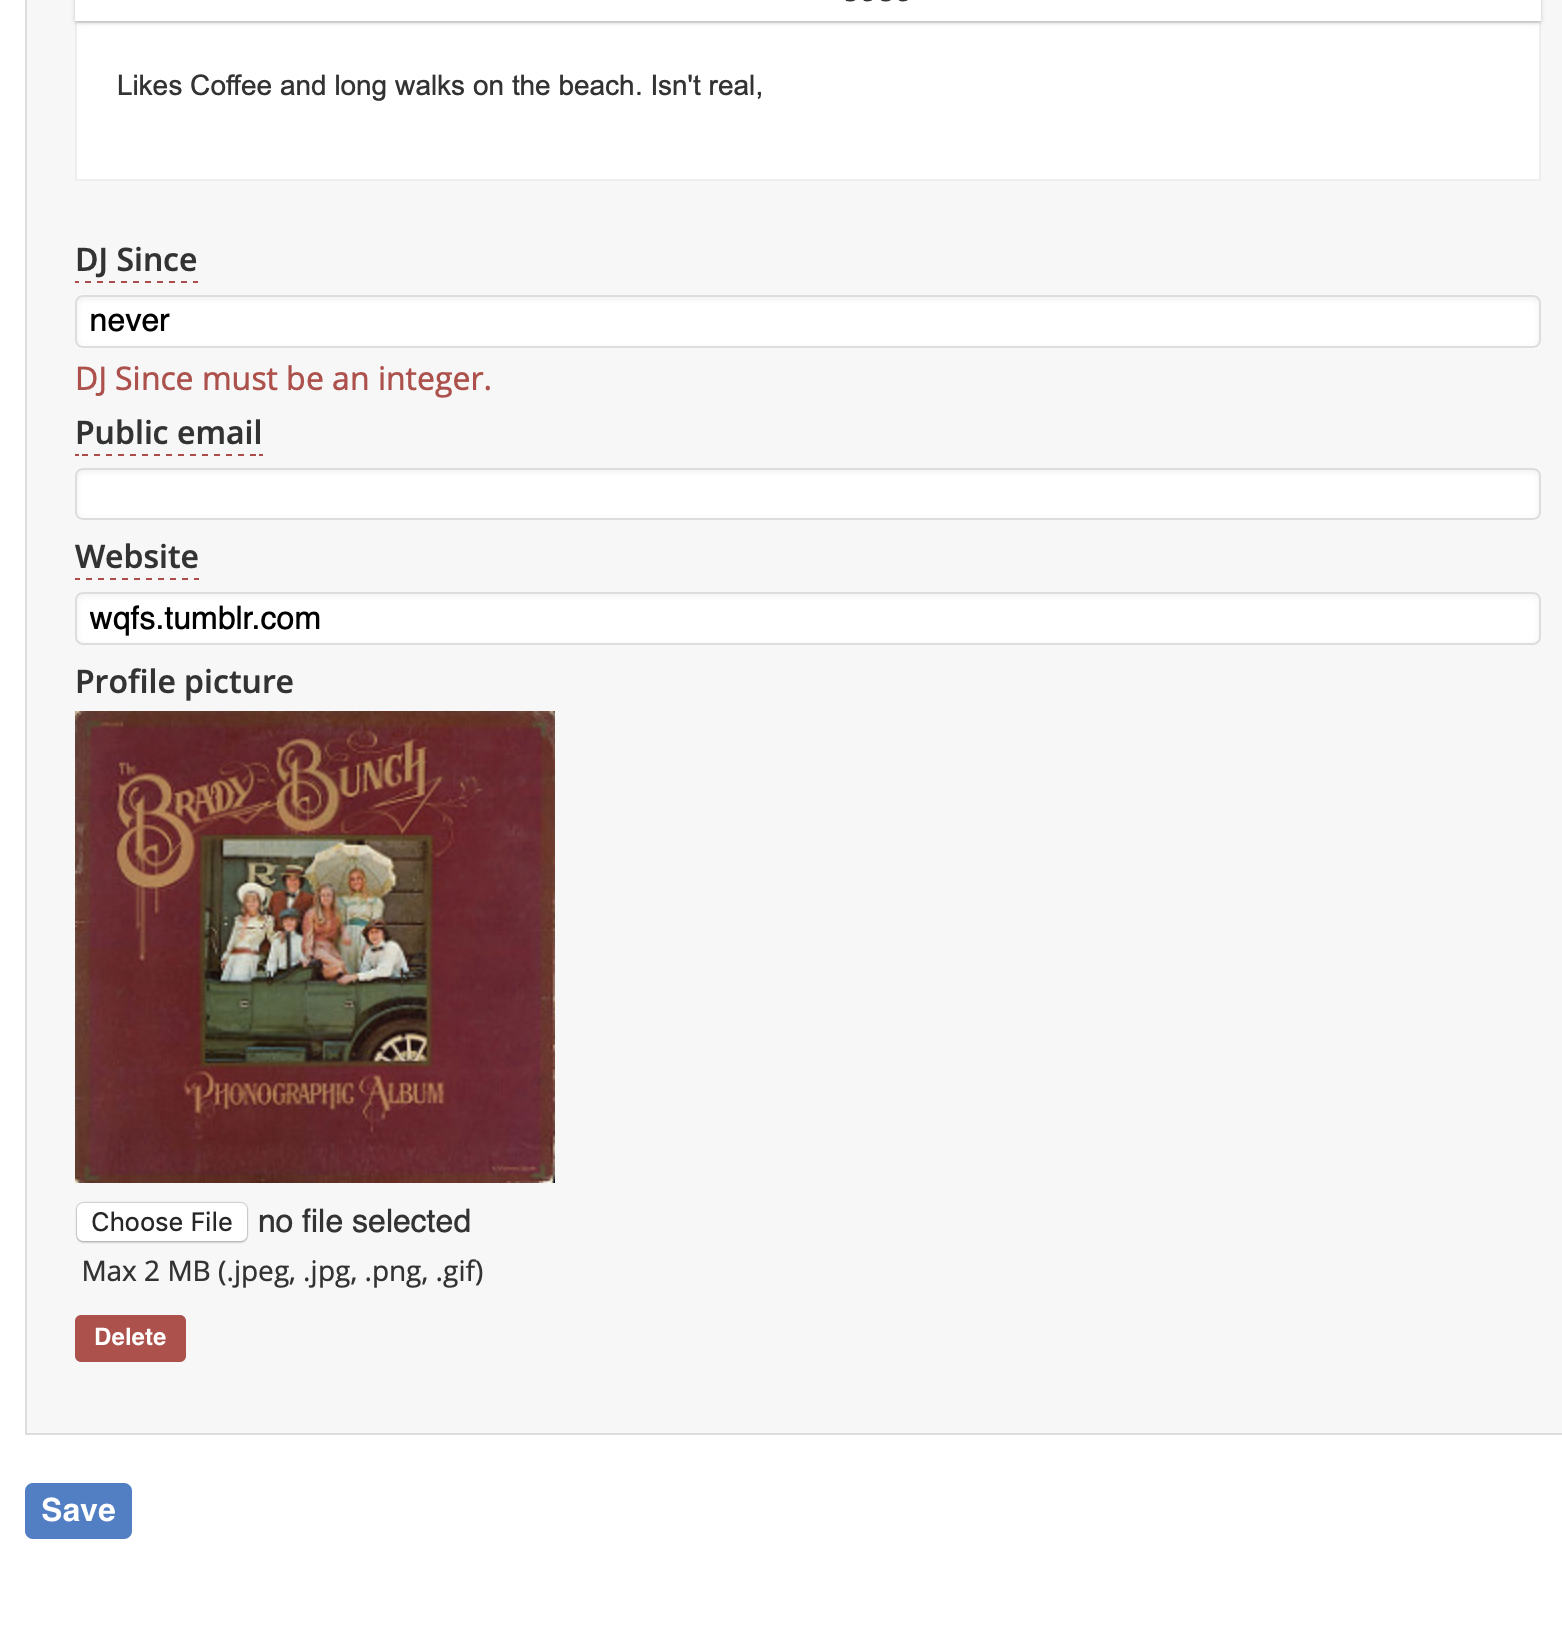
\includegraphics[width=1.0\linewidth, height=5cm]{images/DJ_profile2.png}
%    \label{fig:DJp2}
%    \end{subfigure}
 \caption{This is how spyder looks}
\label{fig6}
\end{figure}



\subsection{Click tab named \textbf{arciguimainrefactored}}
 The Spyder intelligently opens all the previously used programs. In one of the tabs opened by Spyder, a file named \textbf{arciguimainrefactored} shall be present. In case it is not present, the file with the same name shall be found at \path{D/Auto/arci_reformulated/}.All the python files (classes) required to run the program are also present in this folder.
 
 \begin{figure}[H]
 
    \begin{subfigure}{1\textwidth}
    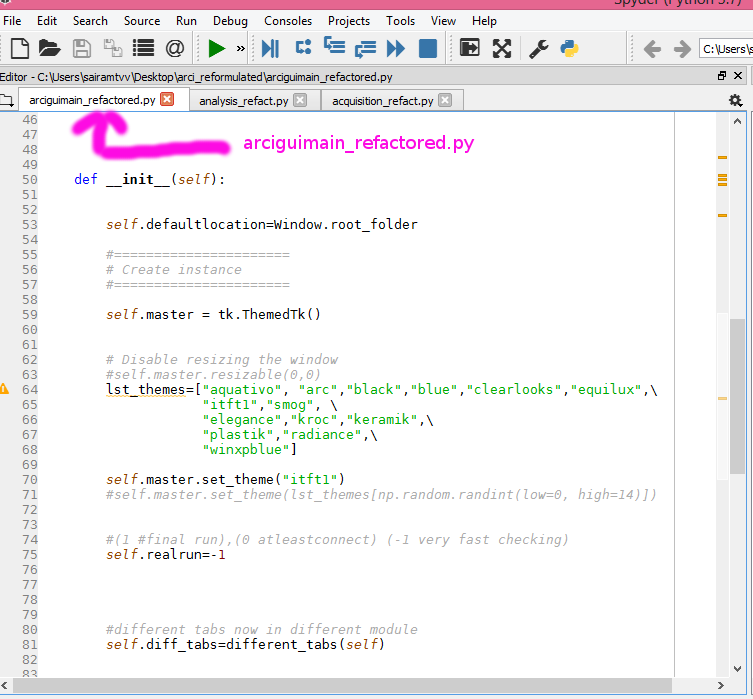
\includegraphics[scale=0.5]{images/arciguimain-refactored.png} 
    \label{fig:DJp1}
    \end{subfigure}
 %   \begin{subfigure}{1\textwidth}
 %   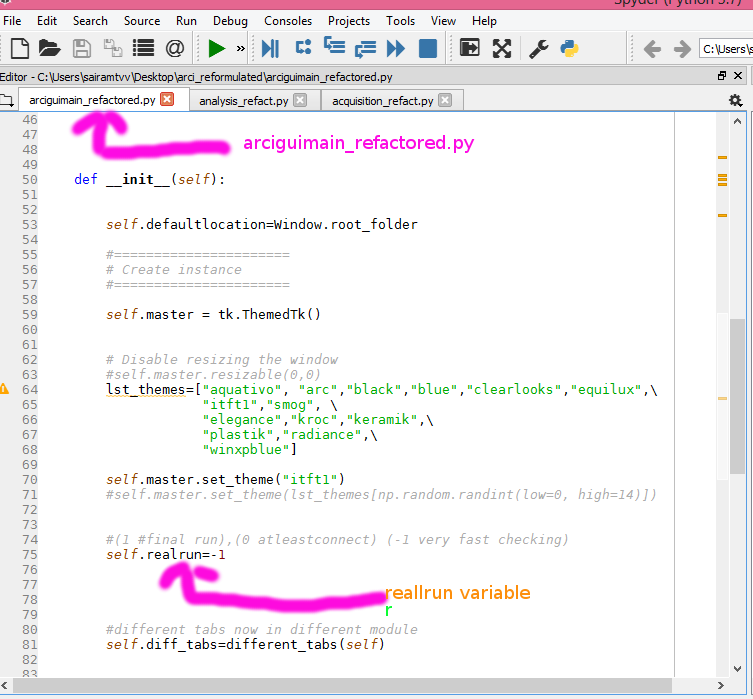
\includegraphics[scale=0.5]{images/realrun.png}
  %  \label{fig:DJp2}
  %  \end{subfigure}
 \caption{The main program tab is highlighted here.}
\label{fig6}
\end{figure}
 
 
\subsection{Choosing Real run variable}
The variable \textbf{real run} can be intelligently varied to suit our need. In case one does not want to meddle with the program they can fix this variable as 1. However, if one wishes to activate only few features to speed up the run. This variable can be changed. 
\begin{enumerate}
    \item realrun=1 (Real run with all delays, connects to all instruments)
    \item realrun=0 (Run without delays, connects to all instruments)
    \item realrun=-1 (For Analysis, does not connect to instruments)
\end{enumerate} 
  
  
  
   
  \begin{figure}[H]
 
    \begin{subfigure}{1\textwidth}
    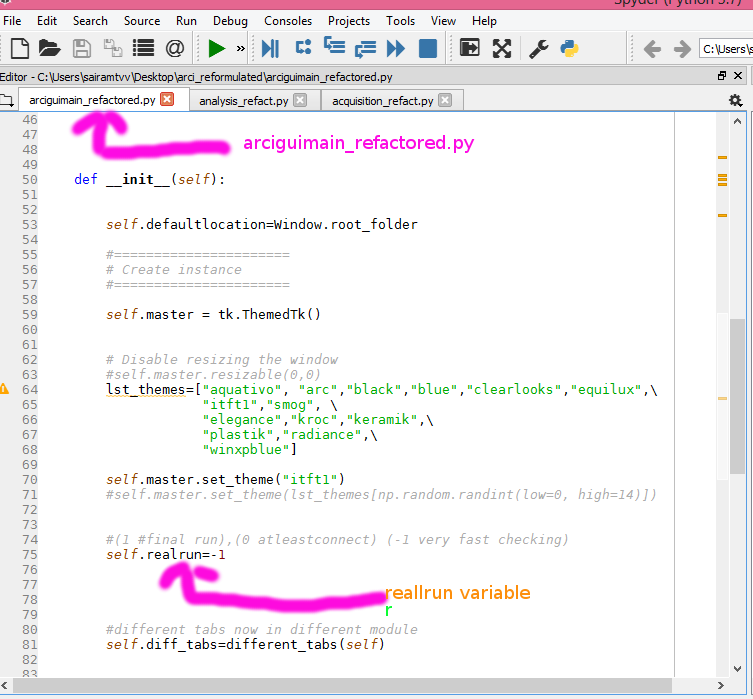
\includegraphics[scale=0.5]{images/realrun.png} 
    \label{fig:DJp1}
    \end{subfigure}
%    \begin{subfigure}{0.5\textwidth}
%    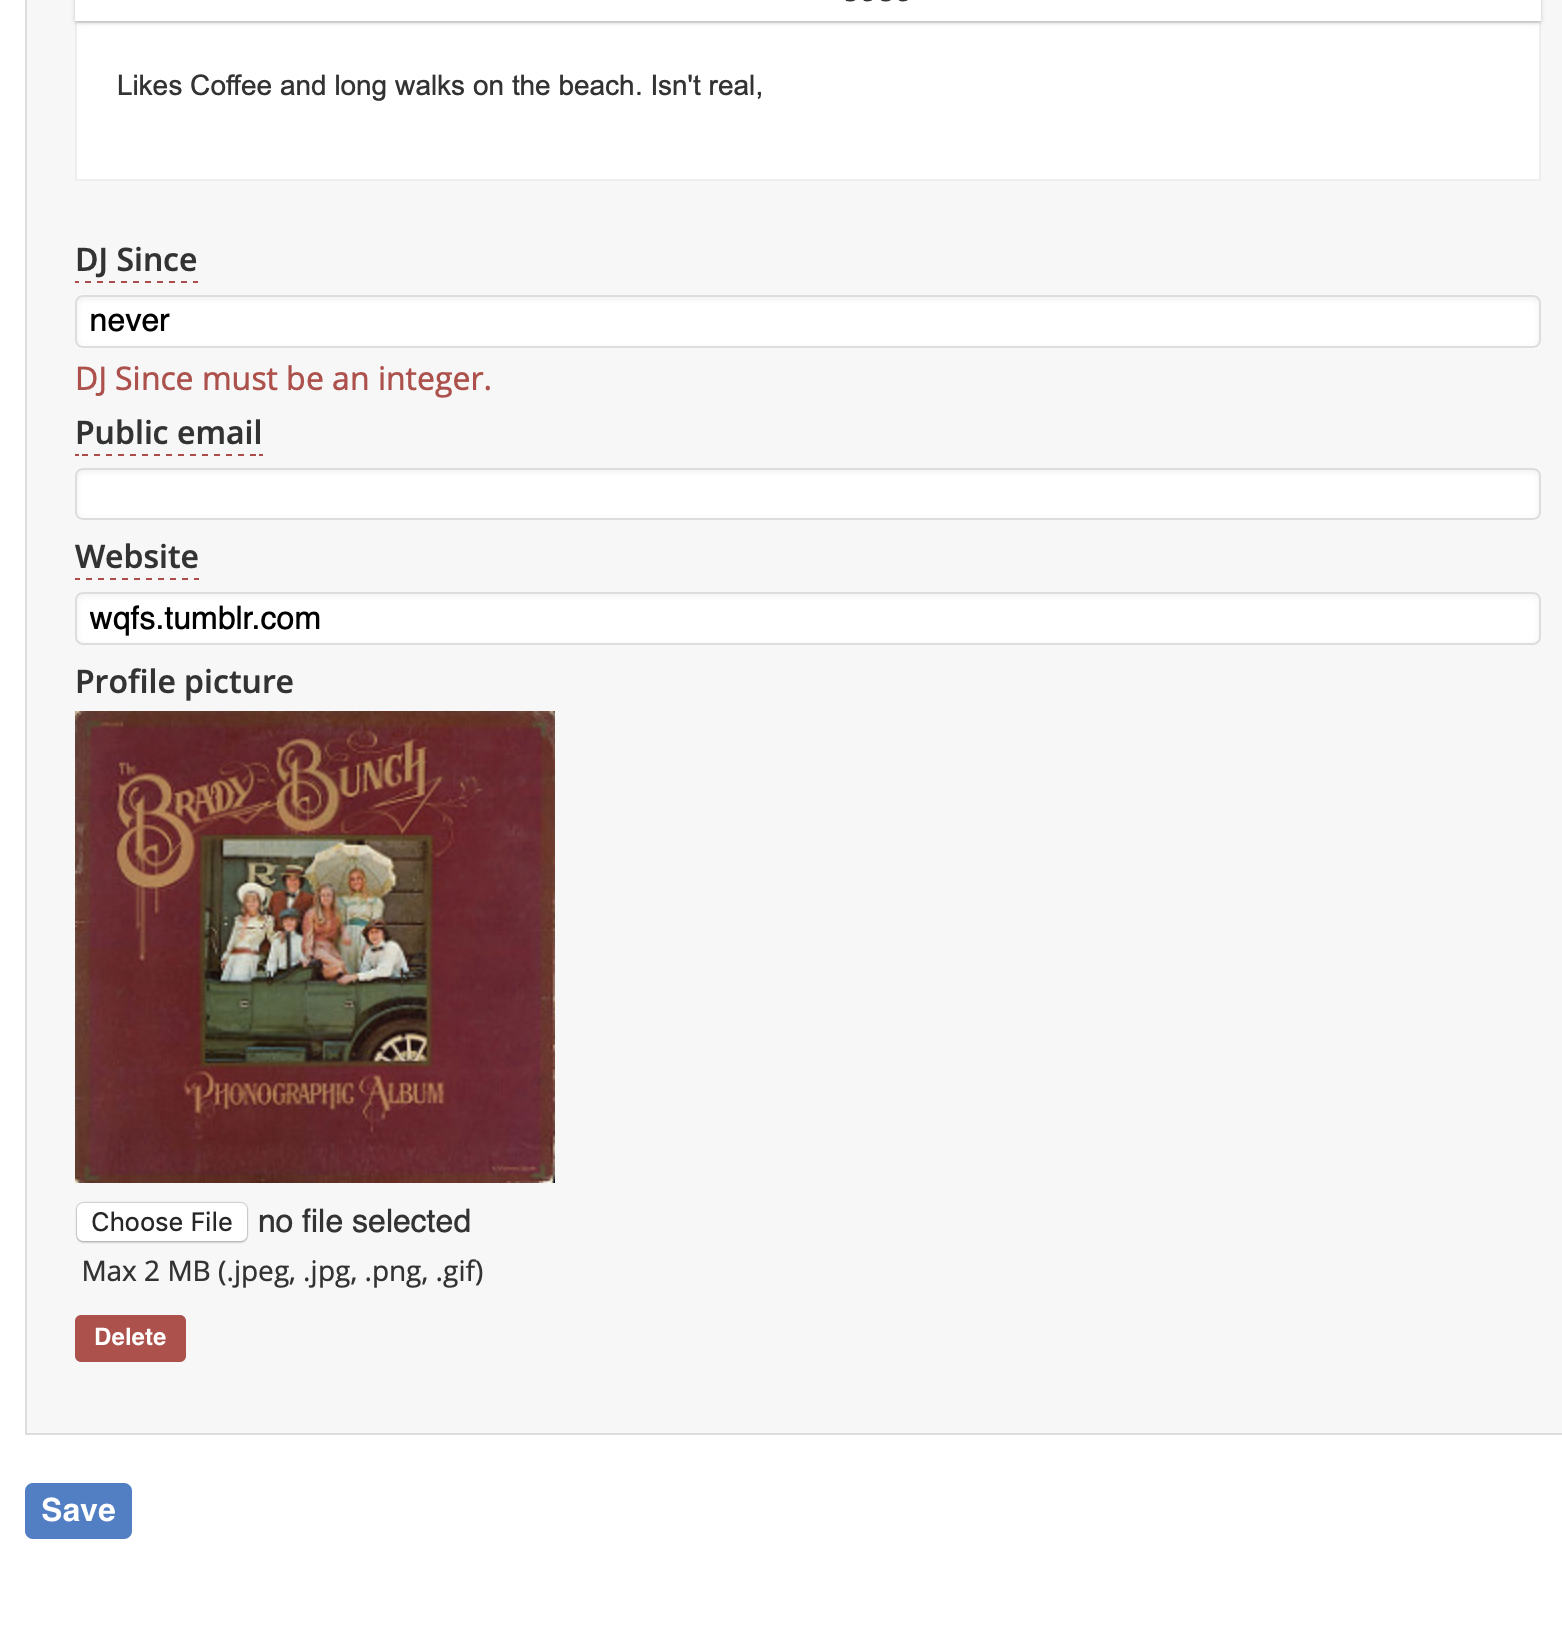
\includegraphics[width=1.0\linewidth, height=5cm]{images/DJ_profile2.png}
%    \label{fig:DJp2}
%    \end{subfigure}
 \caption{The realrun variable is highlighted which is added to provide extra and }
\label{fig6}
\end{figure} 
   
 
 
 \subsection{Open the Bench link data logger3 }
 There is a shortcut of  Bench link data logger3 of agilent present on the desktop. Please press the icon to open the datalogger. After opening the data logger press \textbf{scan and log} tab 
 
 \begin{figure}[H]
    \centering
    \begin{subfigure}{1\textwidth}
    
\includegraphics[scale=4]{images/dataloggericon.png}
    \label{fig:DJp1}
    \end{subfigure}
 %   \begin{subfigure}{1\textwidth}
 %   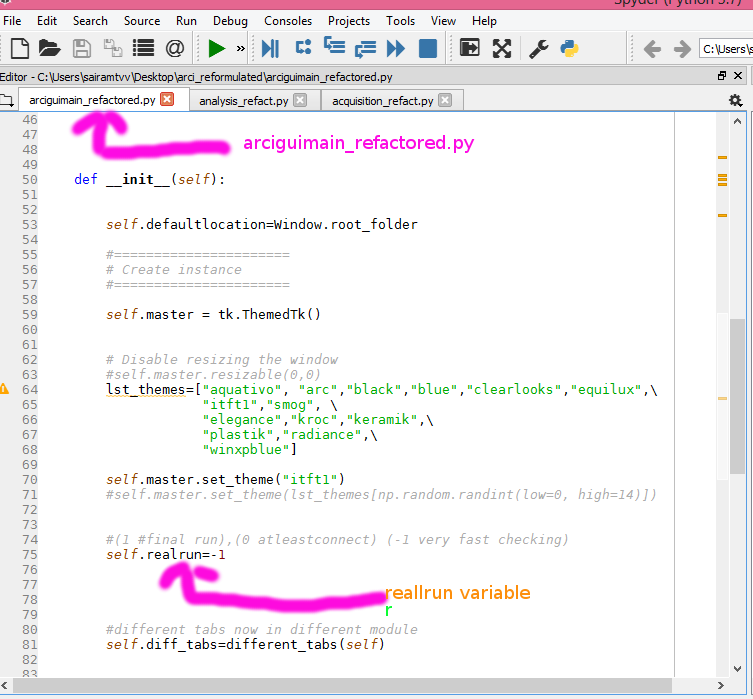
\includegraphics[scale=0.5]{images/realrun.png}
  %  \label{fig:DJp2}
  %  \end{subfigure}
 \caption{This is how the datalogger icon looks on the desktop}
\label{fig6}
\end{figure}
 
 
\subsection{ press the play button in \textbf{arciguimainrefactored}}
Pressing the play button should run the program. 
 
 \begin{figure}[H]
 
    \begin{subfigure}{1.0\textwidth}
    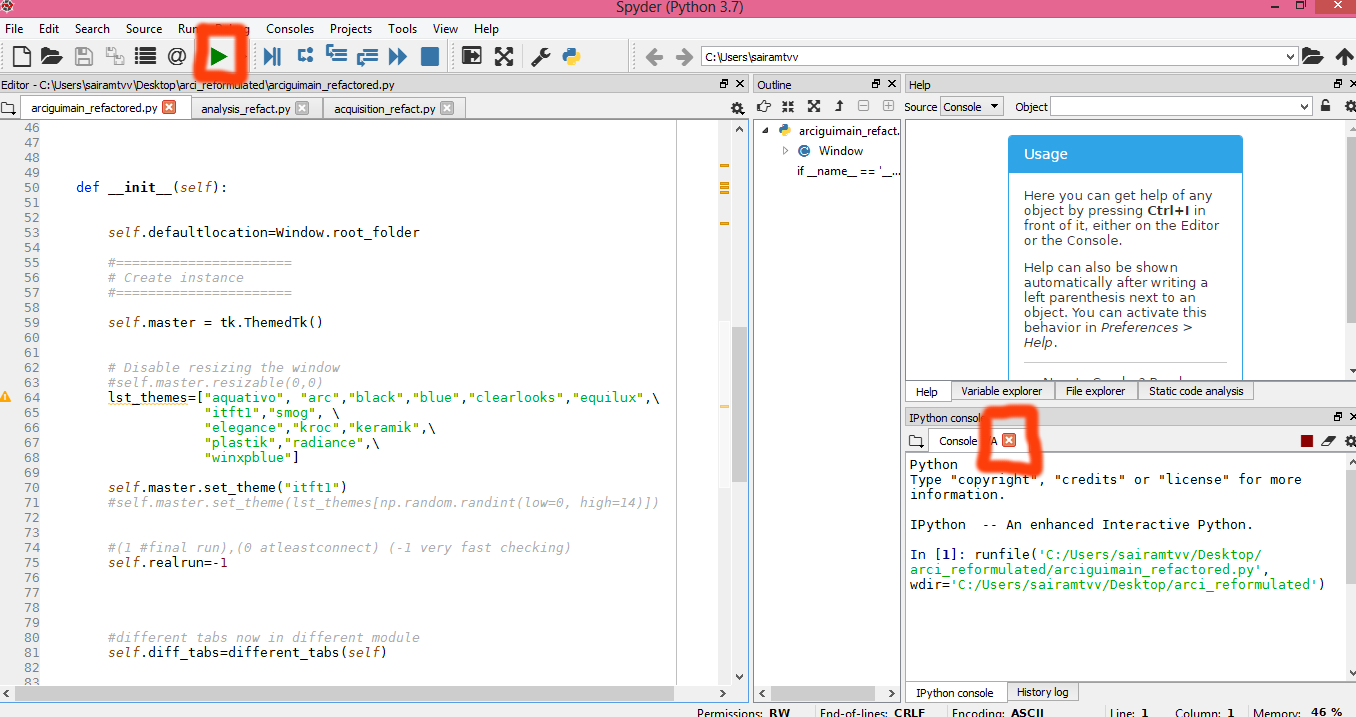
\includegraphics[scale=0.3]{images/playbutton.png} 
    \label{fig:DJp1}
    \end{subfigure}
%    \begin{subfigure}{0.5\textwidth}
%    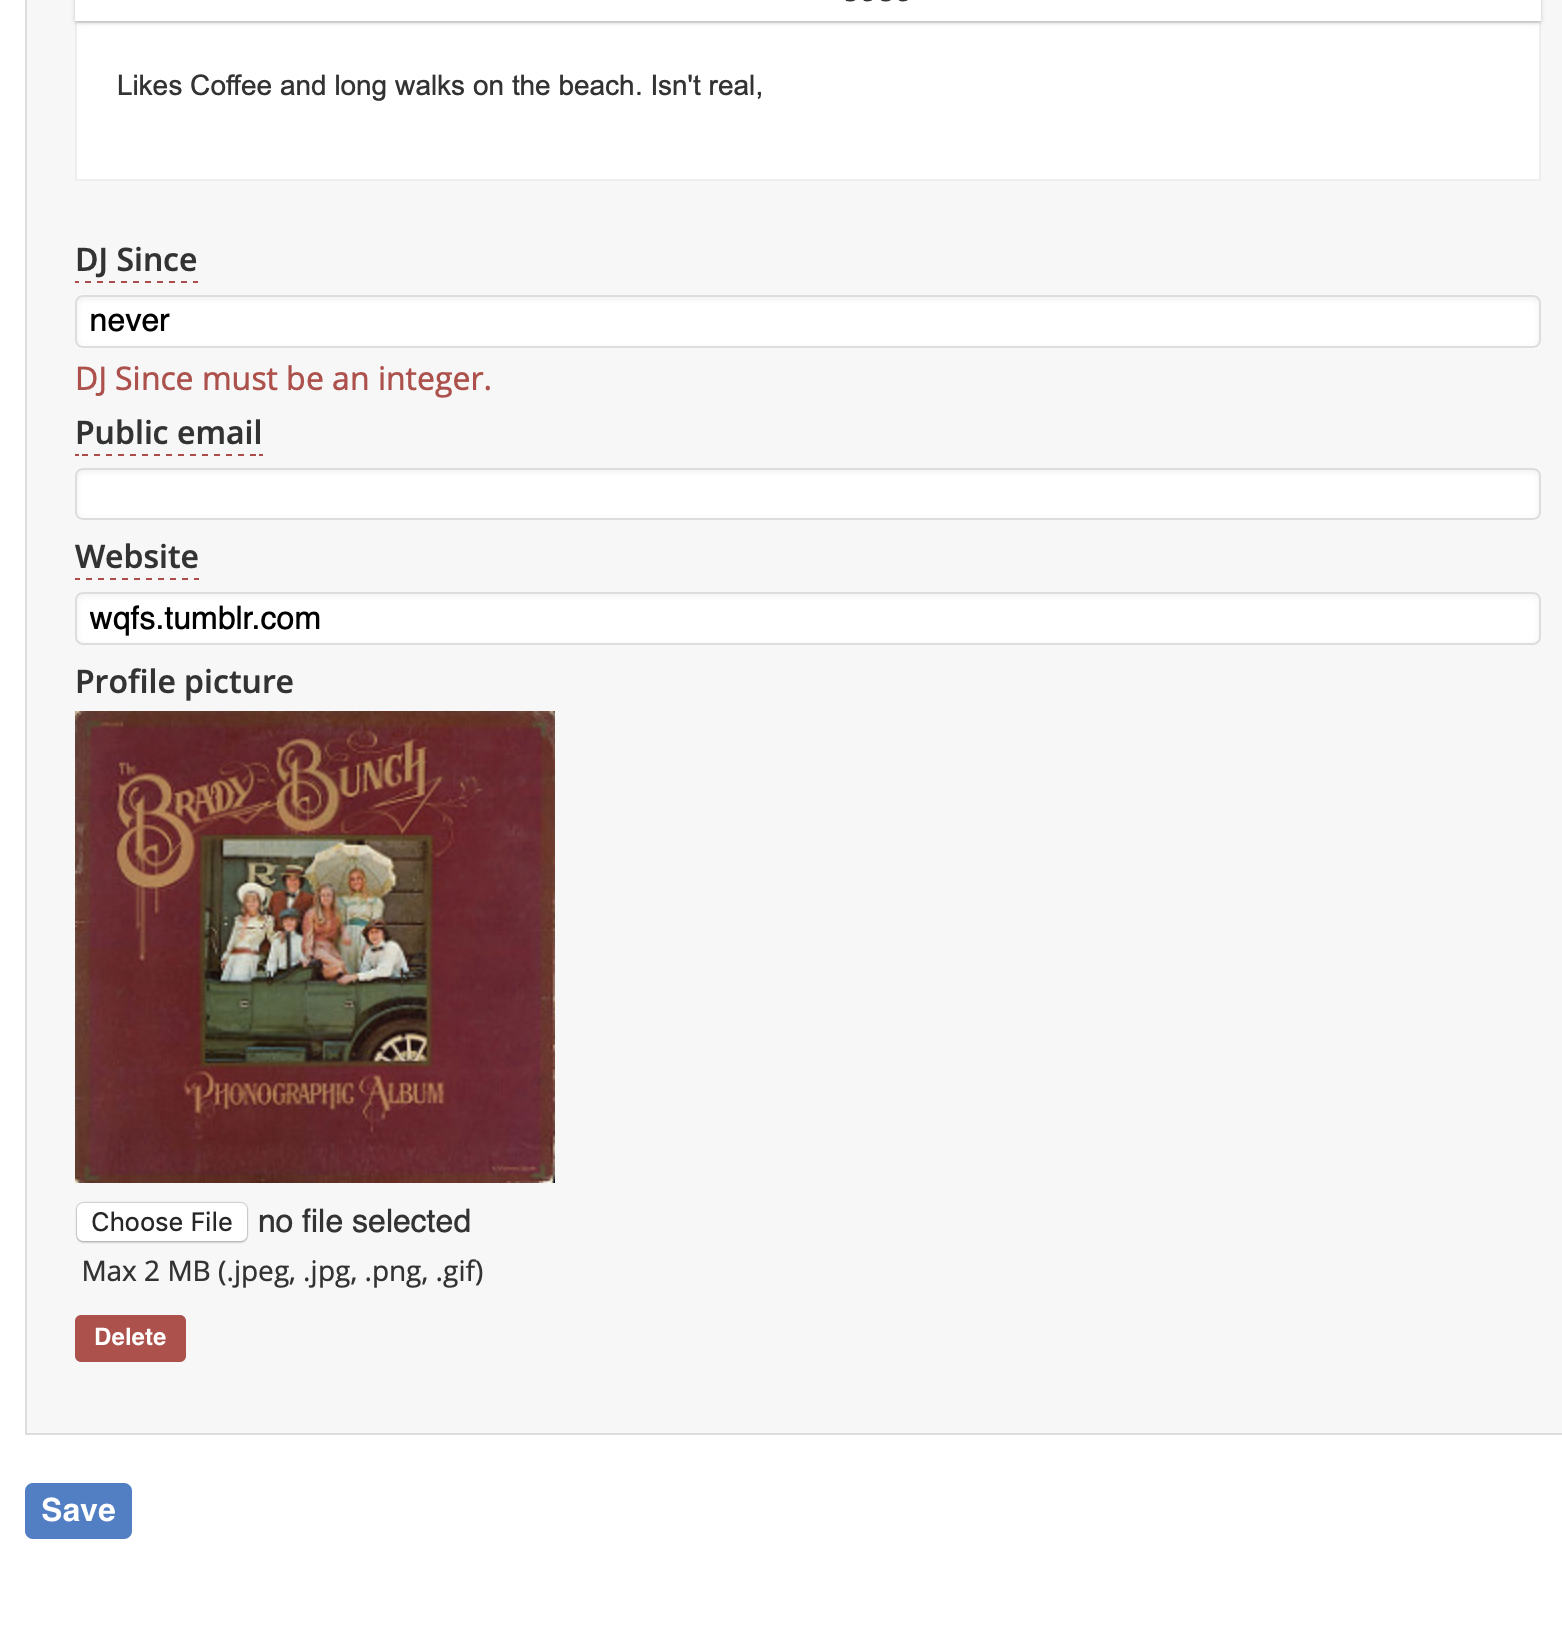
\includegraphics[width=1.0\linewidth, height=5cm]{images/DJ_profile2.png}
%    \label{fig:DJp2}
%    \end{subfigure}
 \caption{Please always press those two marked buttons in red together. Since, parallel programming is invoked for efficiency of the code. It helps in running in a run console.  }
\label{fig6}
\end{figure} 
 
 
 \section{Connecting to the instruments}
 As mentioned earlier, the acquisition  happens only if the value of realrun=0(with no delay between runs) or realrun=1 (real acquisition).The first step always is connecting to the instruments. 
 
 There are three instruments that need to be connected. If any of the instruments are not connected the GUI does not come up. The ip addresses of all the three instruments have been provided to them in a word file.  
 
 \subsection{Connecting to Espec}
 Make sure the ethernet wire is connected between the Espec temperature chamber and the internet switch for the TCP/IP protocol to take place. After the play button has been pressed, it connects and the following message that the connection has been established is shown in the display area. 
 
  
 \begin{figure}[H]
 
    \begin{subfigure}{1.0\textwidth}
    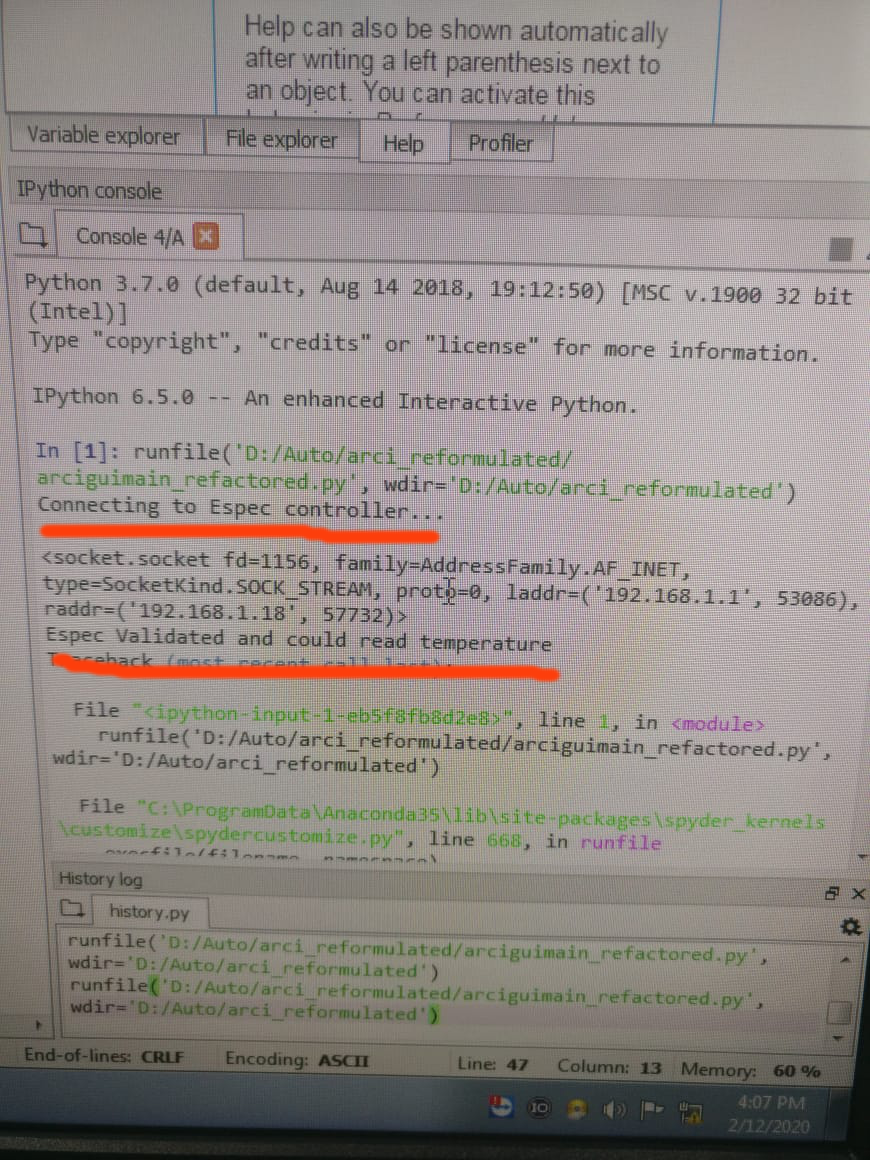
\includegraphics[scale=0.5]{images/espec.png} 
    \label{fig:DJp1}
    \end{subfigure}
%    \begin{subfigure}{0.5\textwidth}
%    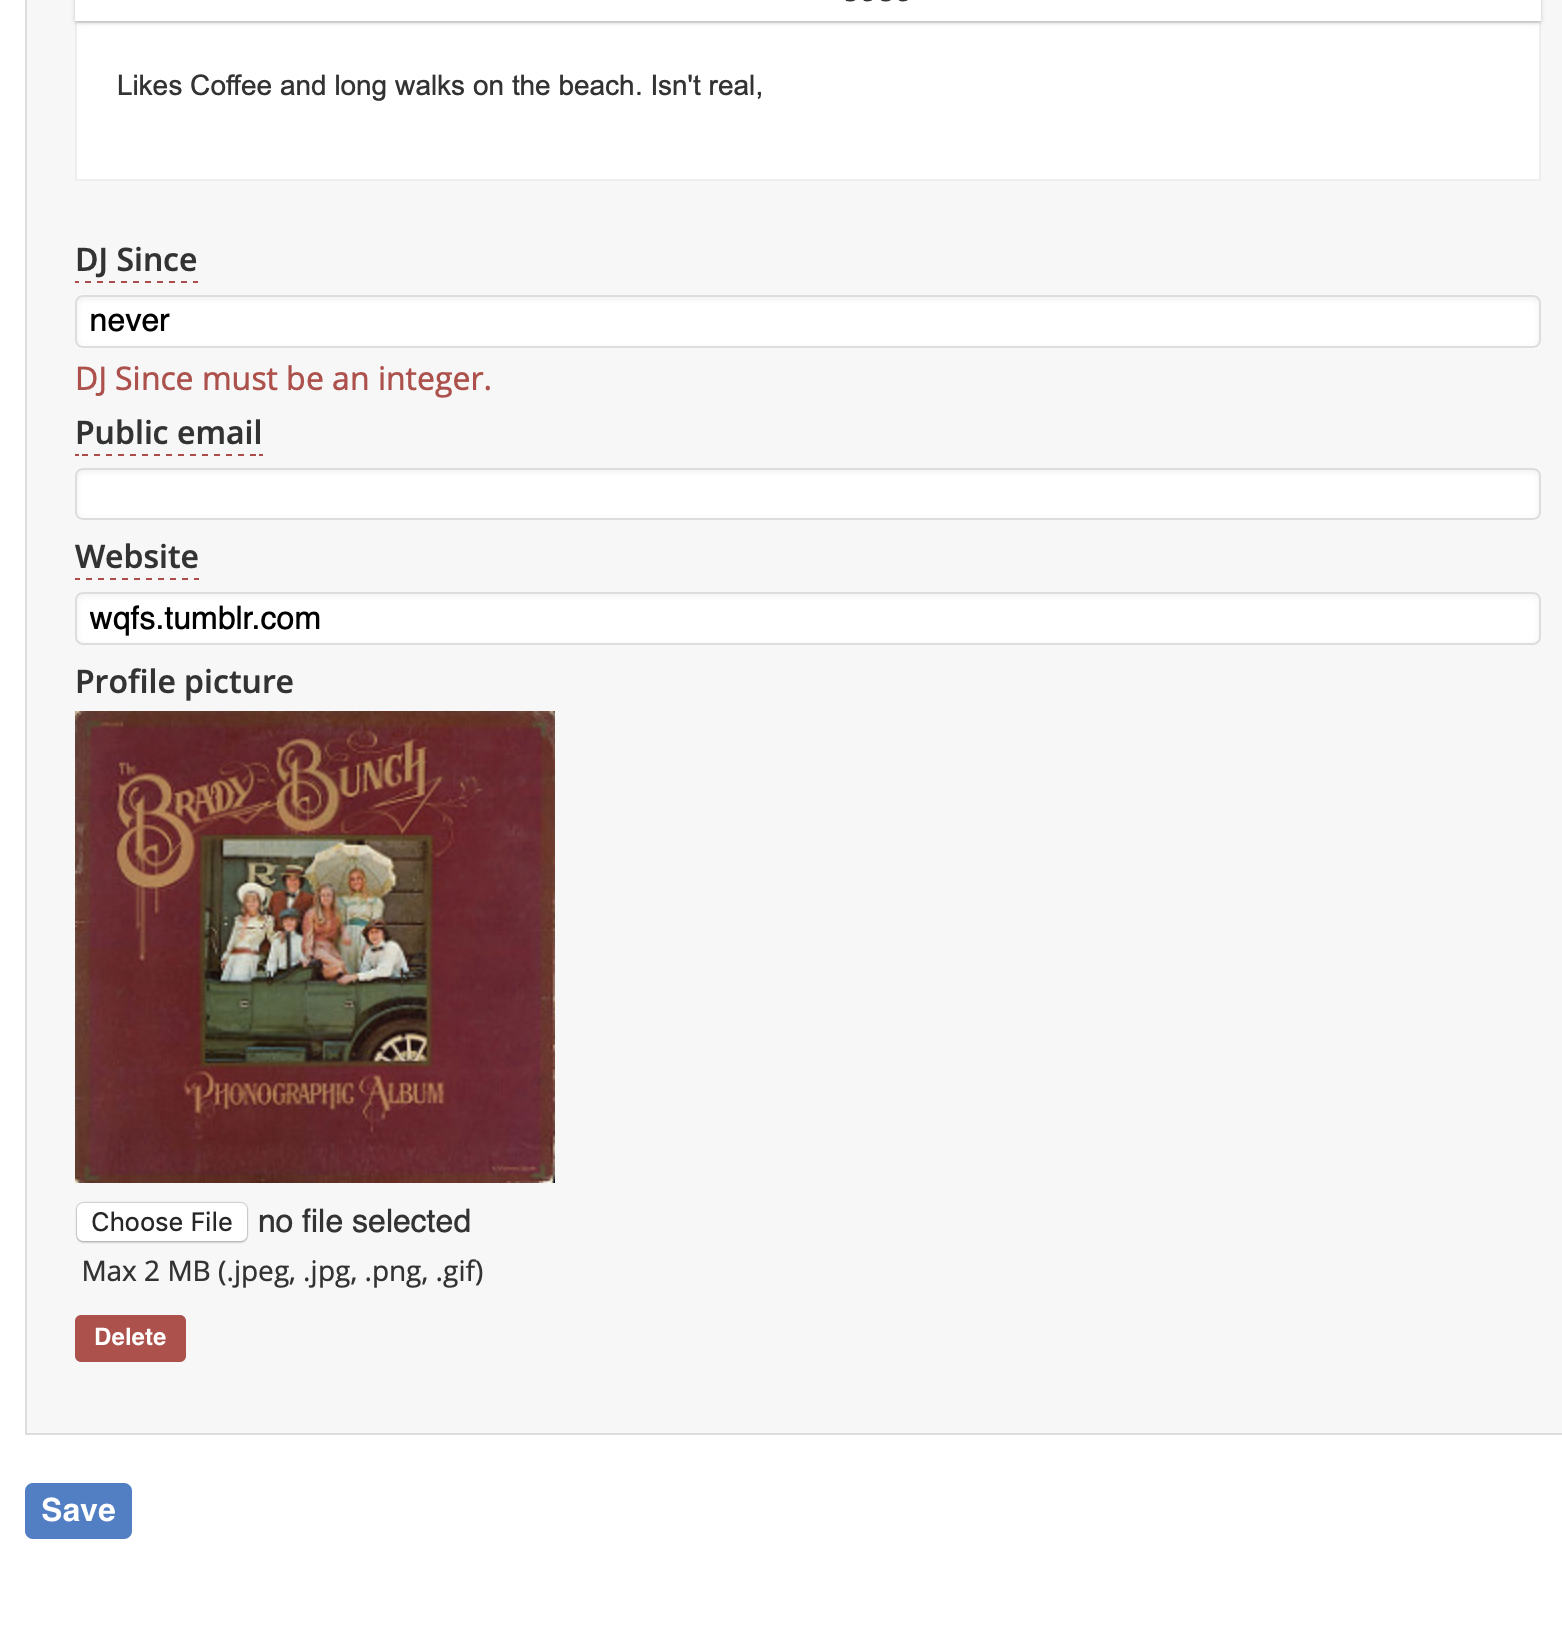
\includegraphics[width=1.0\linewidth, height=5cm]{images/DJ_profile2.png}
%    \label{fig:DJp2}
%    \end{subfigure}
 \caption{The two messages that the software prints out  when espec could be communicated are  connecting to espec, then espec validated and could read temperature are highlighted. }
\label{fig6}
\end{figure} 
 
 Not only it connects to the espec temperature chamber it also takes reads the temperature from the chamber and conveys this information to the user. 
 
 In case the user does not see the above two messages, then probably there is a problem with the hardware connection. Sometimes also rare, it has also been observed that the Espec chamber gets struck. In such moments please restart it by switching off from the plug board also. Only if it reboots, then this struck problem can be resolved.
 
 \subsection{Connecting to Aerotech motion  controller}
 The Aerotech is very particular about the ip addresses. Therefore the ip addresses of the system is set accordingly. It connects to the aerotech controller using chrome. Make sure that you do not update the chrome. In case you update the chrome, then the driver needs to be changed. The following messages are shown when the connection has been established.
 \begin{figure}[H]
 
    \begin{subfigure}{1.0\textwidth}
    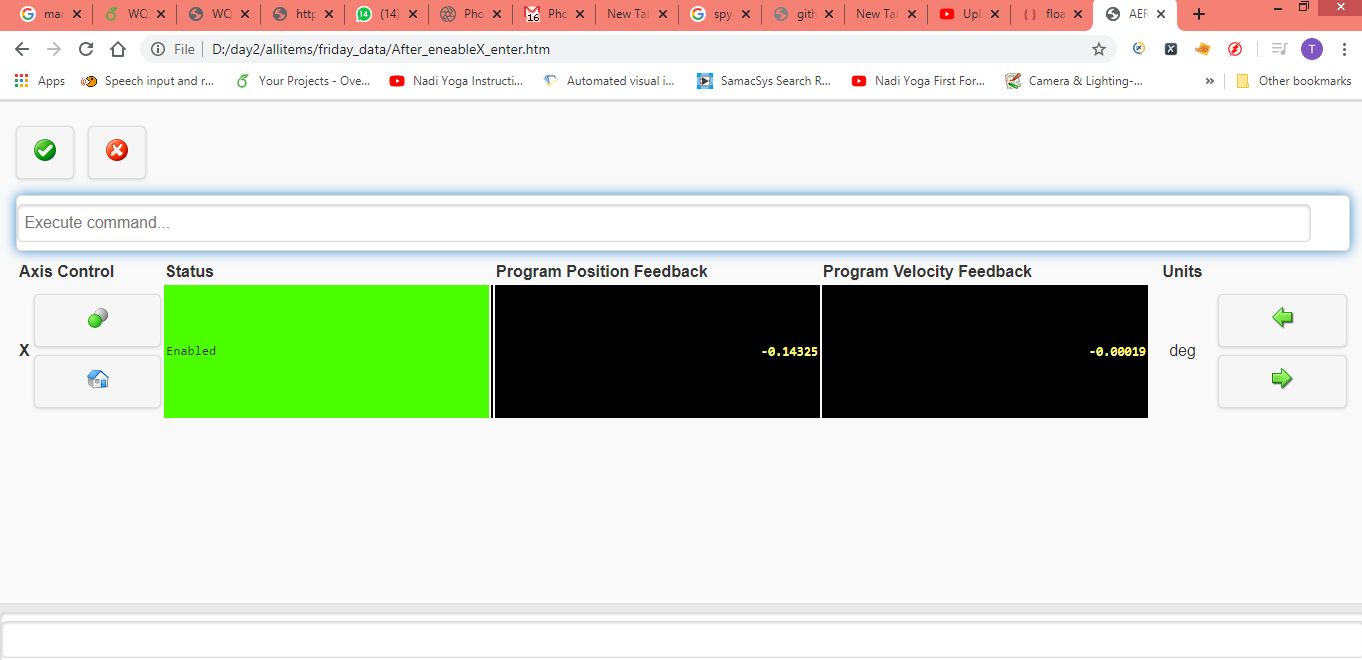
\includegraphics[scale=0.4]{images/aerotech.png} 
    \label{fig:DJp1}
    \end{subfigure}
%    \begin{subfigure}{0.5\textwidth}
%    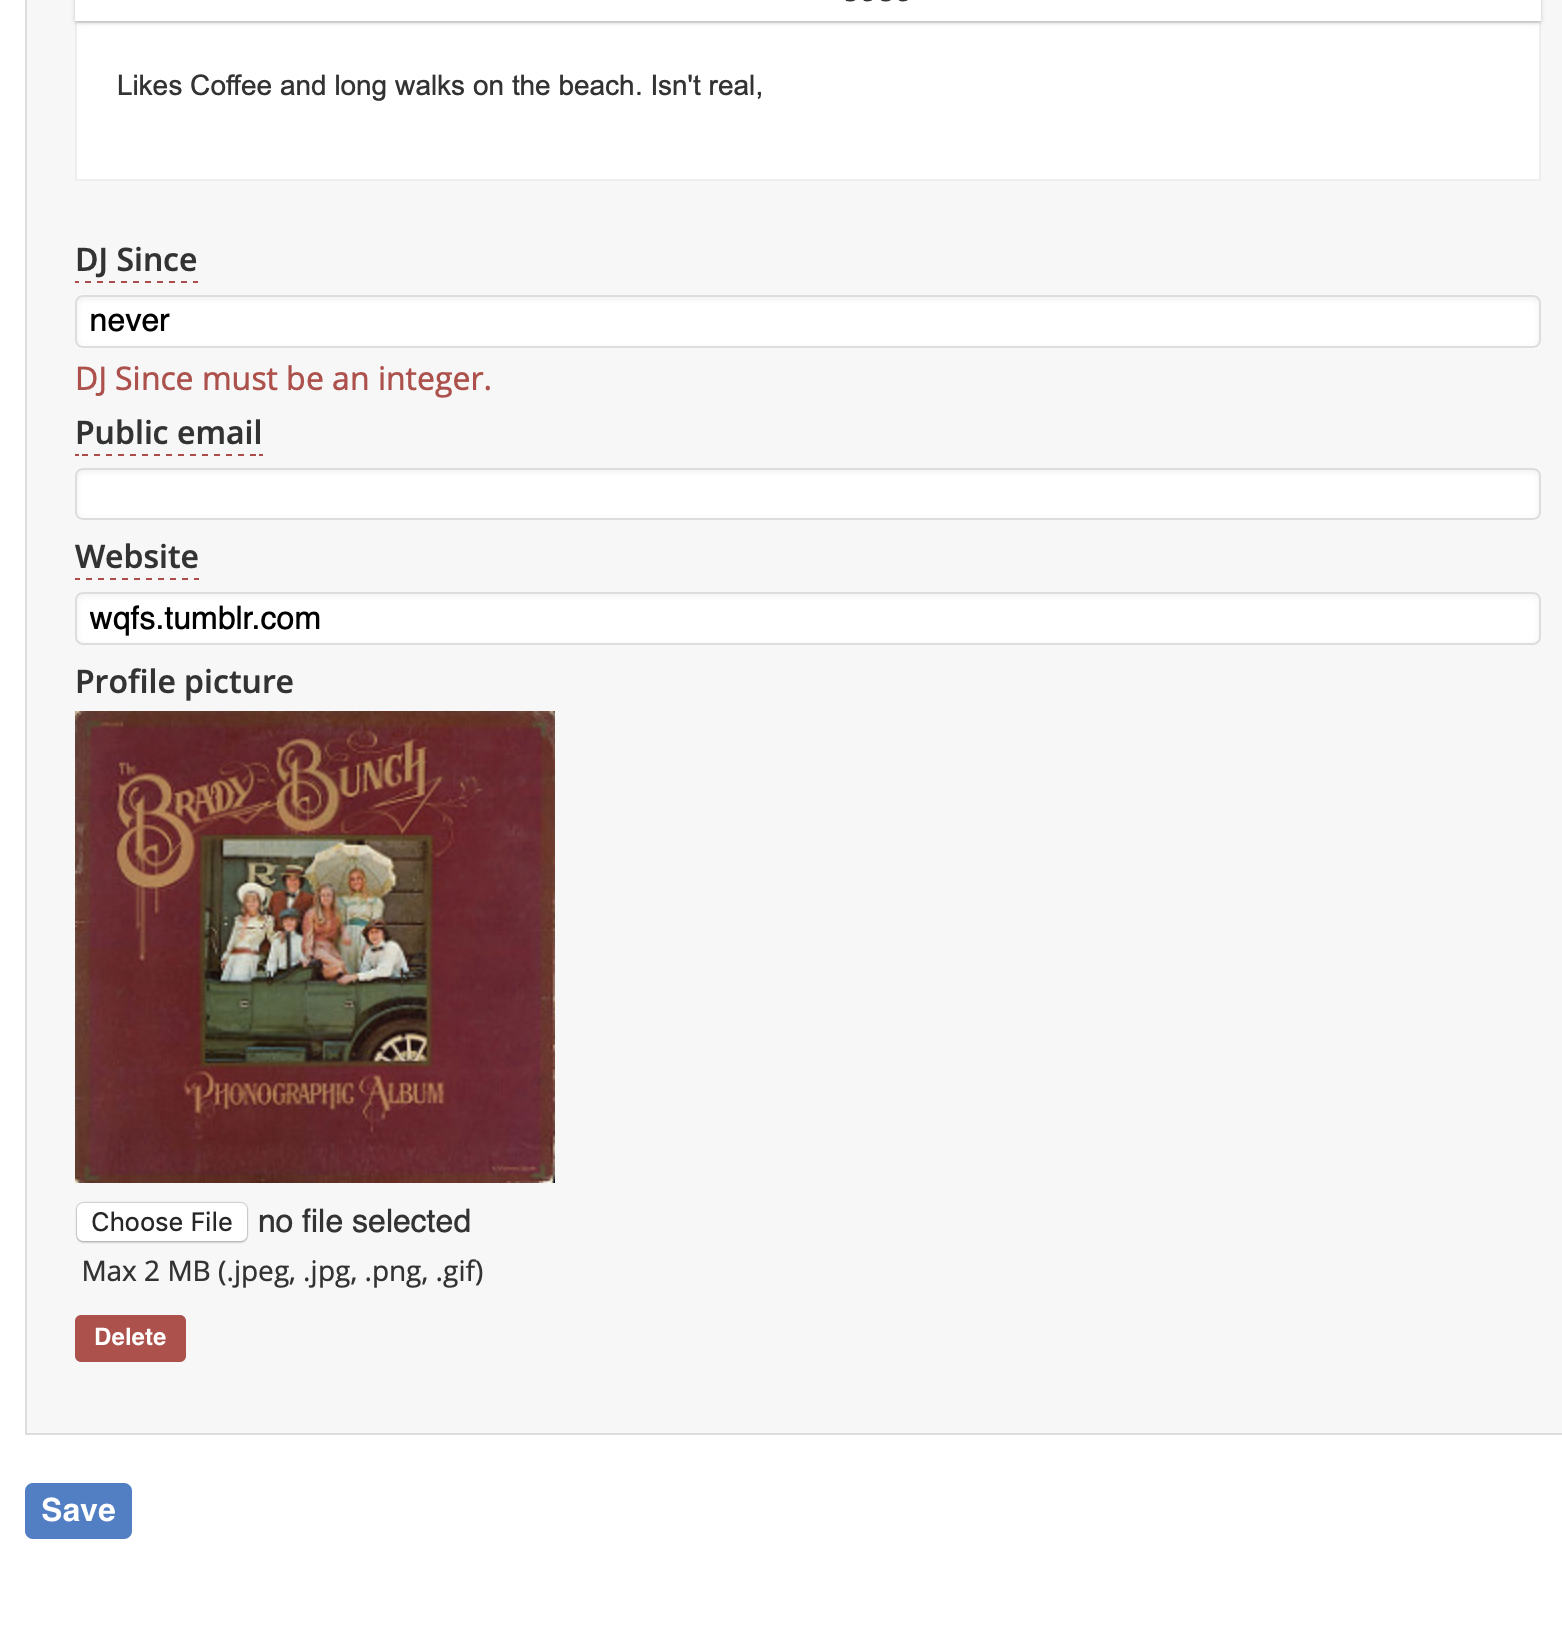
\includegraphics[width=1.0\linewidth, height=5cm]{images/DJ_profile2.png}
%    \label{fig:DJp2}
%    \end{subfigure}
 \caption{The image shown in the figure is automatically opened by chrome browser. That confirms the user that the aerotech connection is suucessful }
\label{fig6}
\end{figure} 
  
 
 After it connects it to the Aero-tech position controller, the following functionalities shall be activated
 
 \begin{enumerate}
     \item It activates the X-direction motion  if it is not already activated
     \item It Homes the system and waits for 60 seconds
     
 \end{enumerate}
 
After these check ups when it is sure that it can connect to Aerotech position controller, it starts connecting to the Agilent Data Logger.
 
 
  \subsection{Connecting to Agilent Datalogger}
 we have discussed earlier about opening the Agilent Data logger and pressing the Scan and log tab. Now the program establishes  a connection with Agilent switch using RS-232 protocol. Then, it acquires some dummy data to check whether data acquisition can happen happen or not from Agilent switch. 
 
 \begin{figure}[H]
 
    \begin{subfigure}{1\textwidth}
    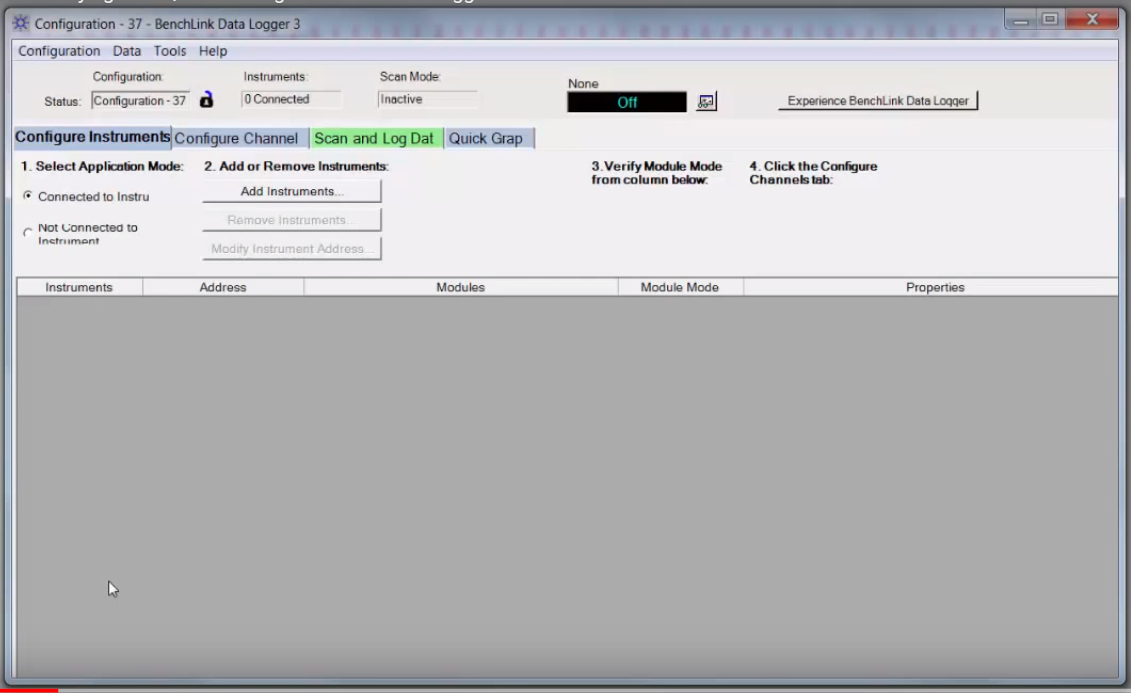
\includegraphics[scale=0.5]{images/datalogger_front.png} 
    \label{fig:DJp1}
    \end{subfigure}
%    \begin{subfigure}{0.5\textwidth}
%    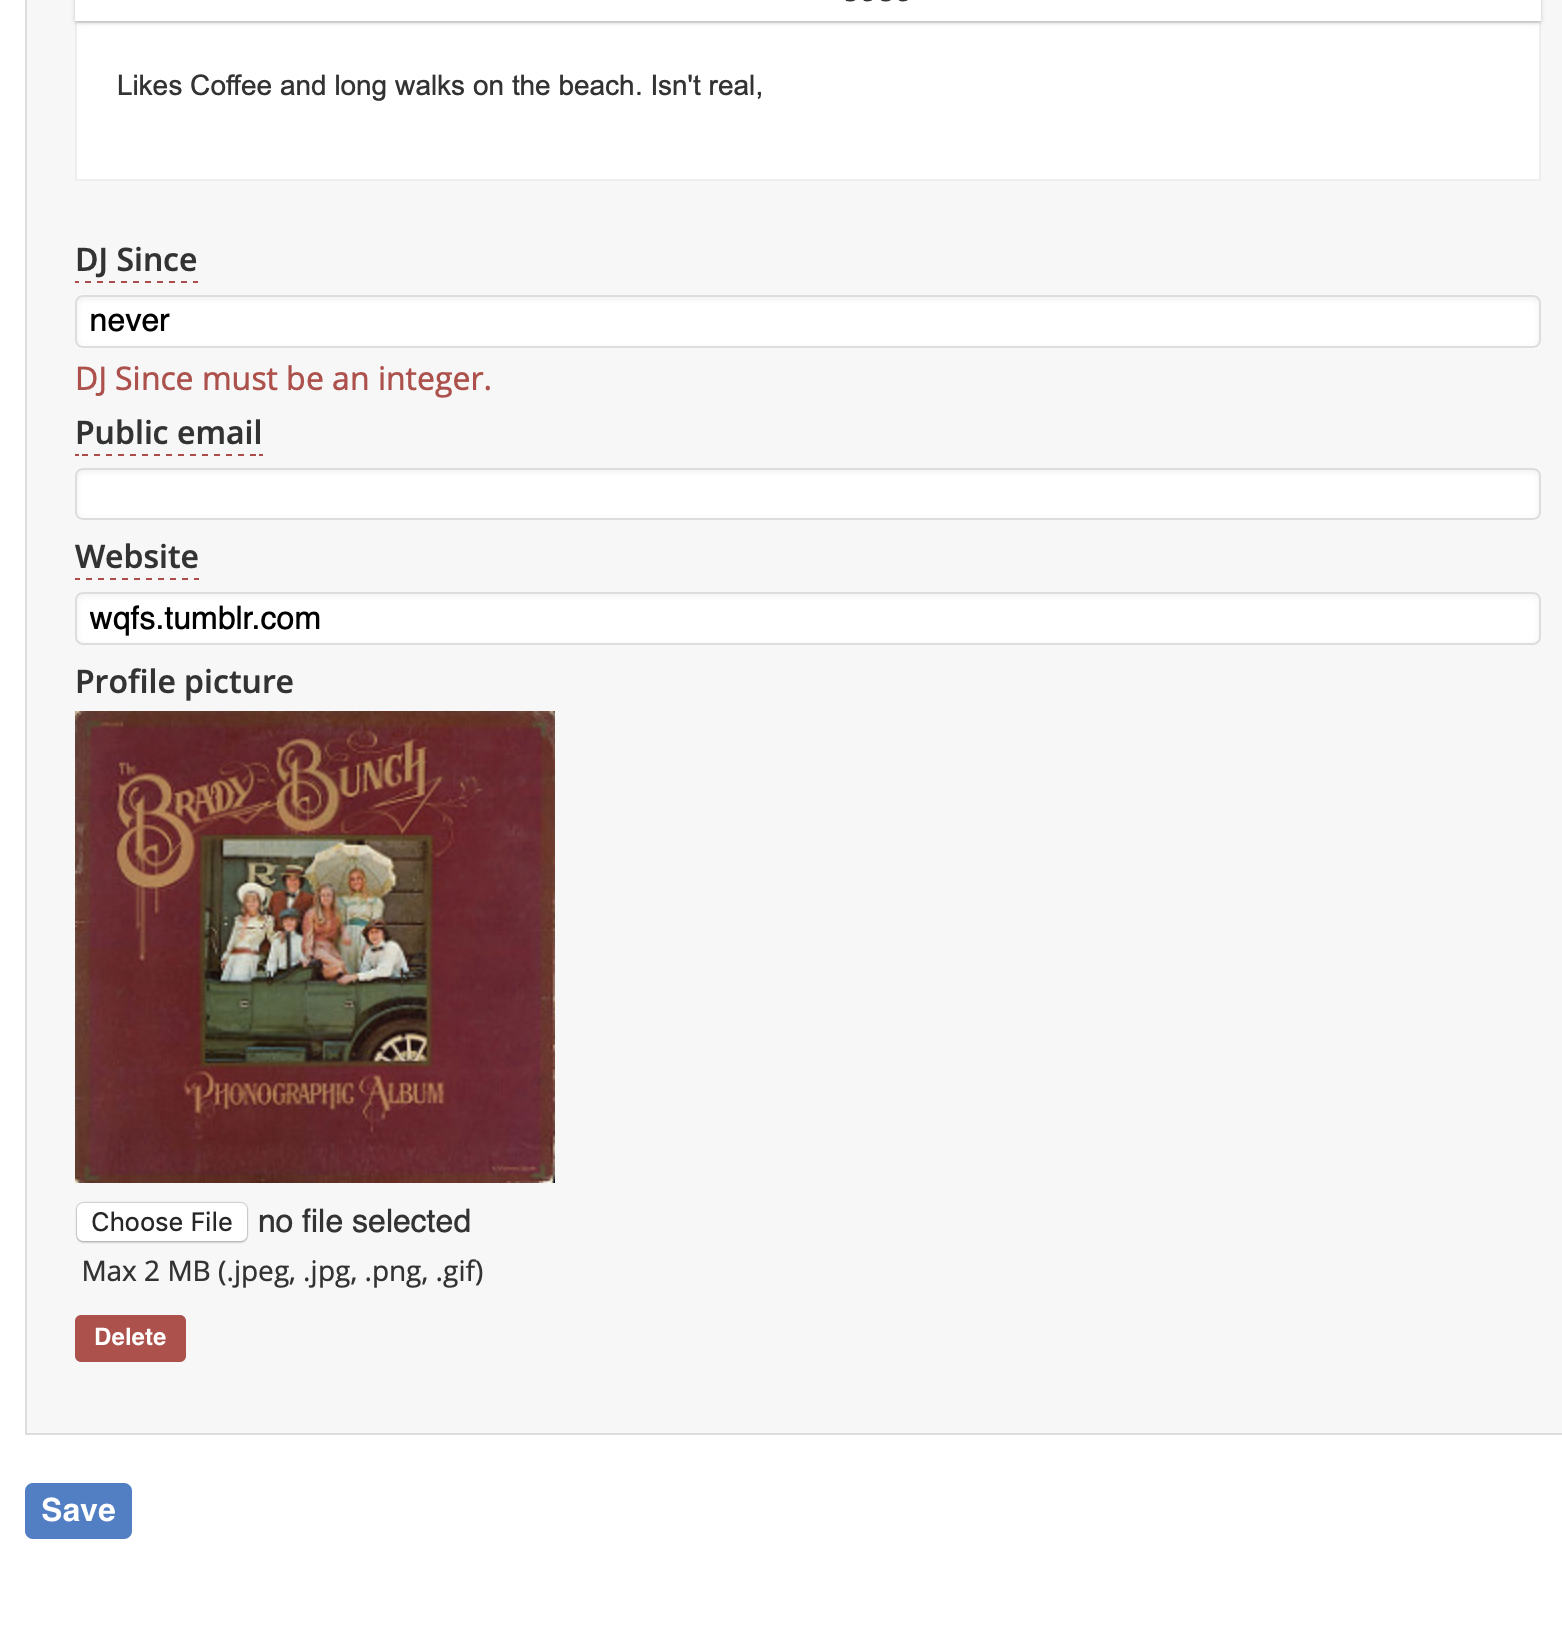
\includegraphics[width=1.0\linewidth, height=5cm]{images/DJ_profile2.png}
%    \label{fig:DJp2}
%    \end{subfigure}
 \caption{This is how the Agilent data logger looks after opening it }
\label{fig6}
\end{figure} 
 
 
 Once a successful acquisition of data happens from Agilent switch. A Graphical user Interface (GUI) appears where all the tasks required can be performed with few clicks.
 
 \section{Description of GUI}
 GUI was designed after understanding their complete sequence which spans over 6 days. There are different blocks in the GUI catering to different aspects of the experiment. The moment the GUI screen is visible   
 
 \subsection{Assigning Sensor names}
  
    \subsubsection{Run name}
     This is a very important variable. This decides the name of the folder which all the six days data shall be stored. It is very important to note that for all the six days the name of  this variable should be same, only then the data of all the days shall be collected into this folder. In case, the name of Run name is different as given from  the first day (L1) and if such a name is not present, then it results in an error, saying please check the folder name as such a folder does not exist
   
   
   \begin{figure}[H]
 
    \begin{subfigure}{1.0\textwidth}
    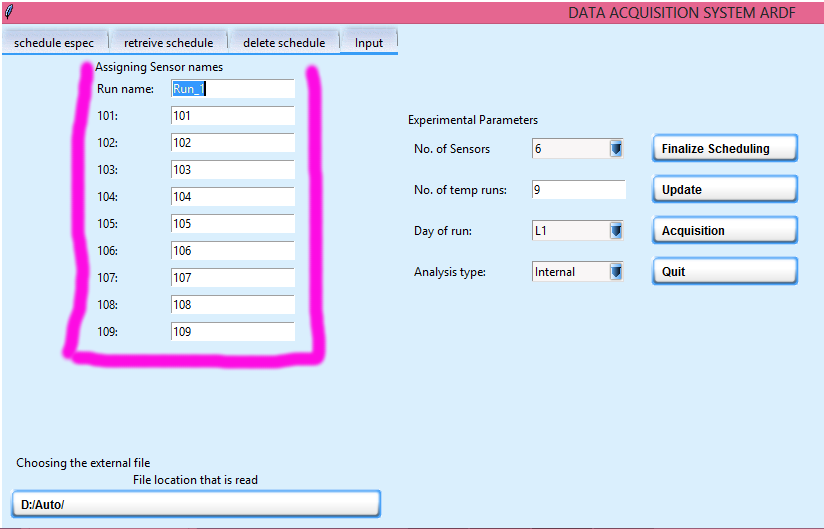
\includegraphics[scale=0.5]{images/assigning_sensor_names.png} 
    \label{fig:DJp1}
    \end{subfigure}
%    \begin{subfigure}{0.5\textwidth}
%    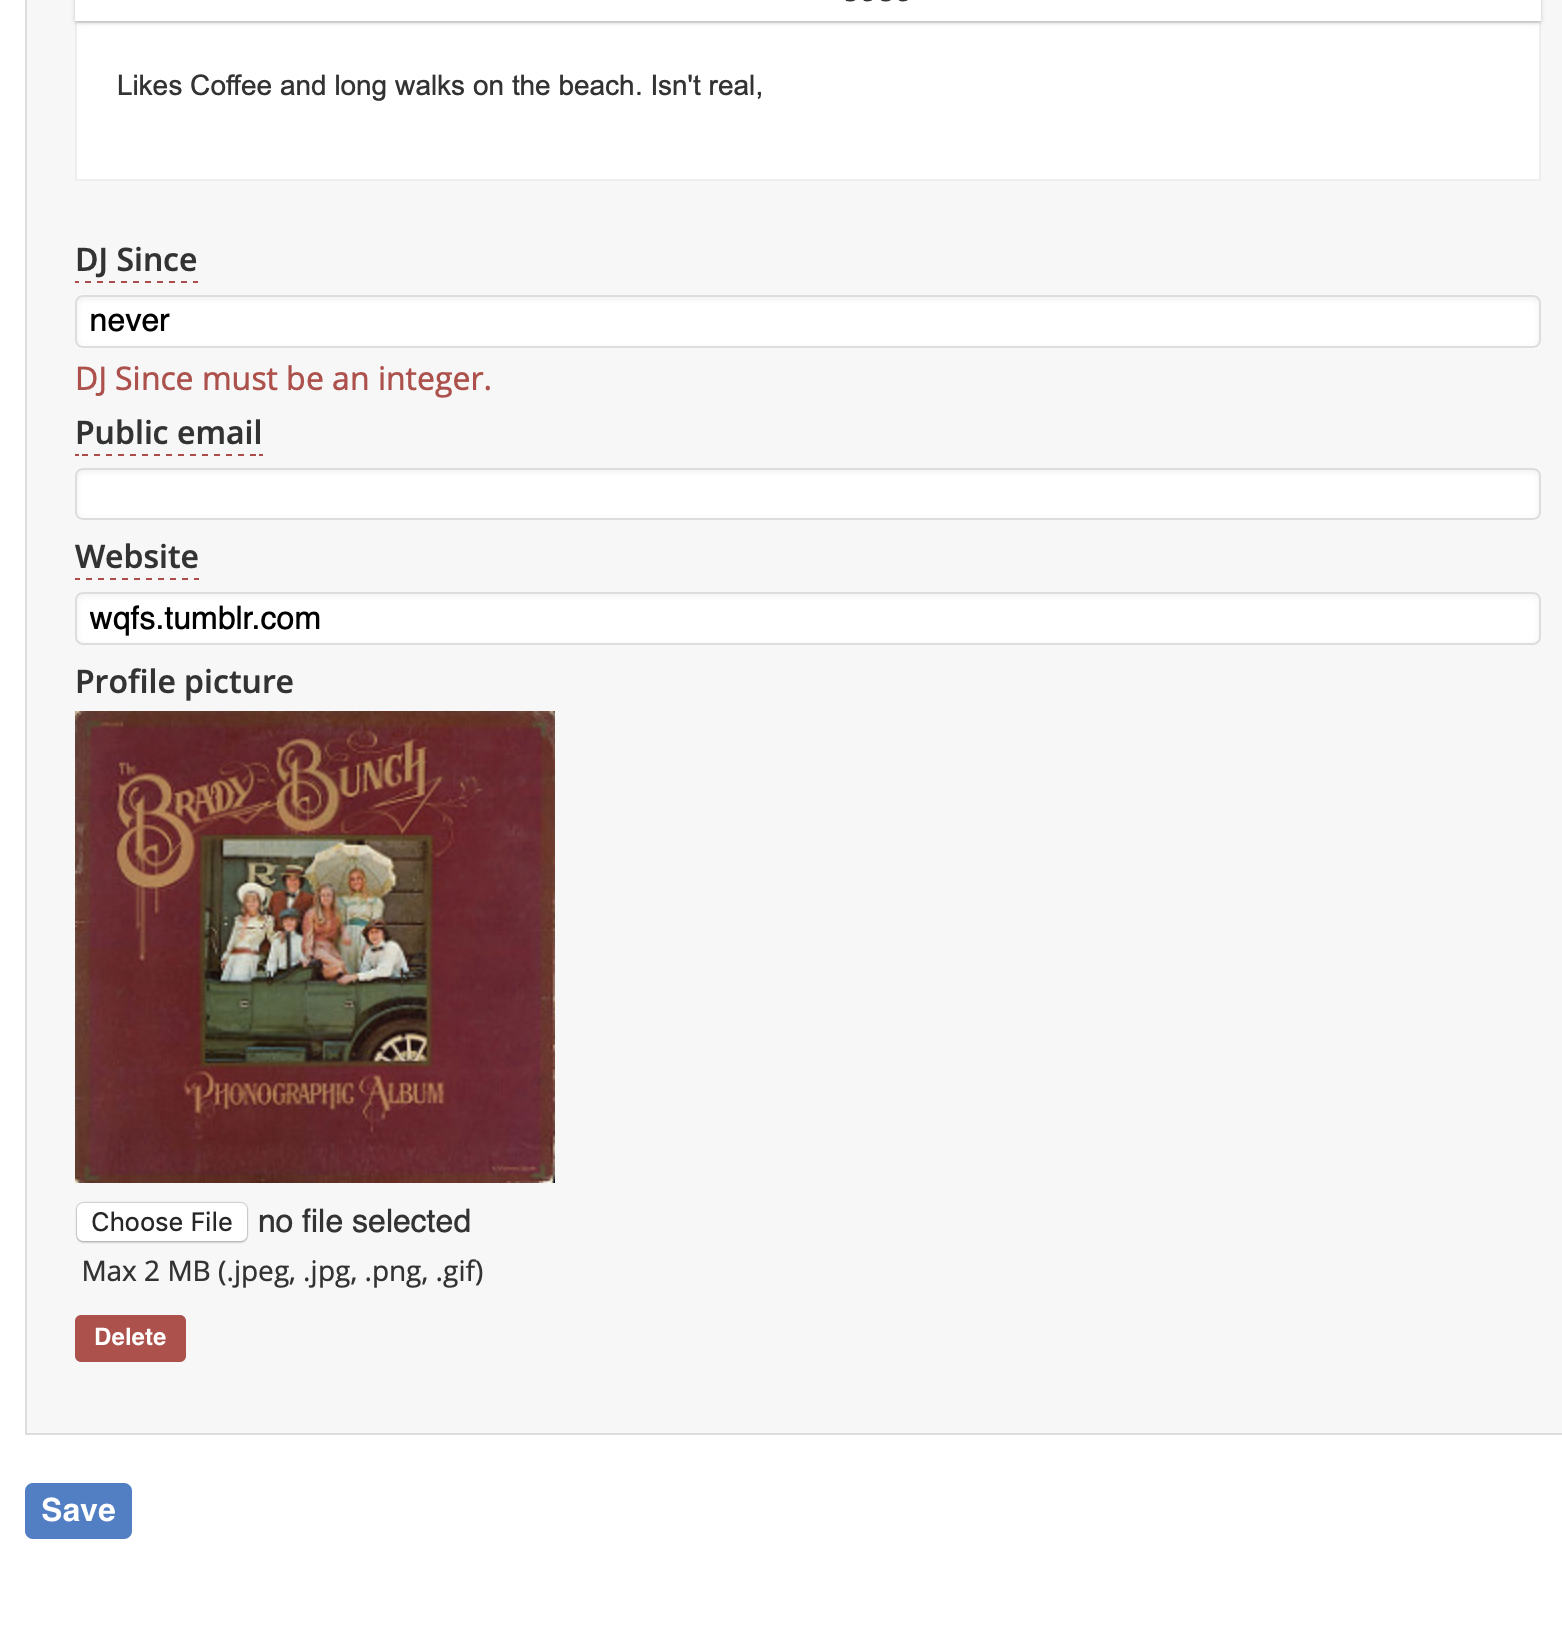
\includegraphics[width=1.0\linewidth, height=5cm]{images/DJ_profile2.png}
%    \label{fig:DJp2}
%    \end{subfigure}
 
 \caption{Highlighted the Run name and sensor names section}
\label{fig6}
\end{figure}
   
   
   
    
    
    
    
    \subsubsection{Sensor names}
    Actually, the names of these sensors does not matter when you are acquisition. These names that are assigned turn up as folders and all the information regarding the respective sensor are stored into it. Therefore, the names of these sensors becomes very important during the Analysis phase 
    \begin{enumerate}
        \item 101: Name of the first sensor
        \item 102: Name of the second sensor
        \item ...
        \item ....
        \item ...
        \item ....
        \item ...
        \item ....
        \item 109: Name of the ninth sensor
    \end{enumerate}
    Thus nine sensors can be accommodated here.
    
\subsection{Experimental Parameters}
These are the most important parameters and decides the course of the experiment. These parameters were designed and the control was given to user as variation of these variables deemed necessary.

    \subsubsection{Number of Sensors}
    By default the value of this variable is set to 6 which are the maximum amount of sensors that can be placed inside the Espec temperature chamber. By default the software acquires data from all the six channels. But this parameter becomes important during analysis phase. 
    
    \subsubsection{Number of temperature runs}
    These are the number of temperature runs in the L1, L2 and L3 cycle. By default it is 9. However, they can varied. Be sure that the number of the temperature runs given during the acquisition should be same as the analysis.
    
    
    \begin{figure}[H]
 
    \begin{subfigure}{1.0\textwidth}
    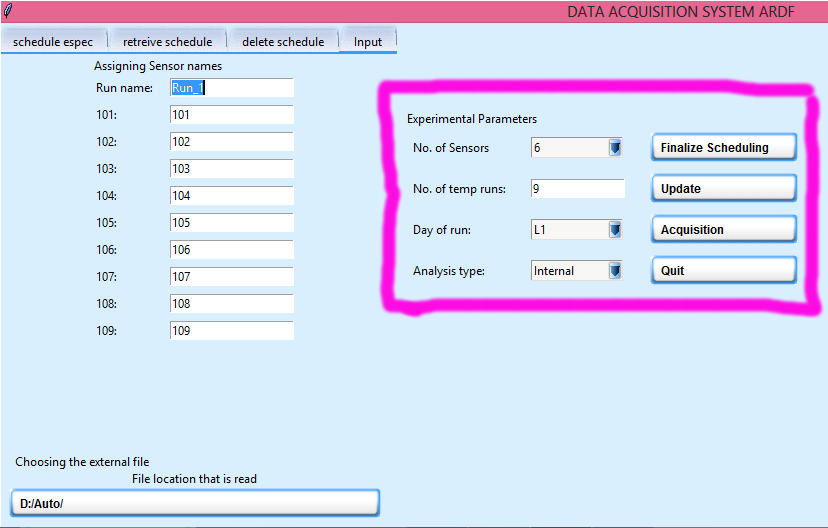
\includegraphics[scale=0.5]{images/experiemntal_parameters.png} 
    \label{fig:DJp1}
    \end{subfigure}
%    \begin{subfigure}{0.5\textwidth}
%    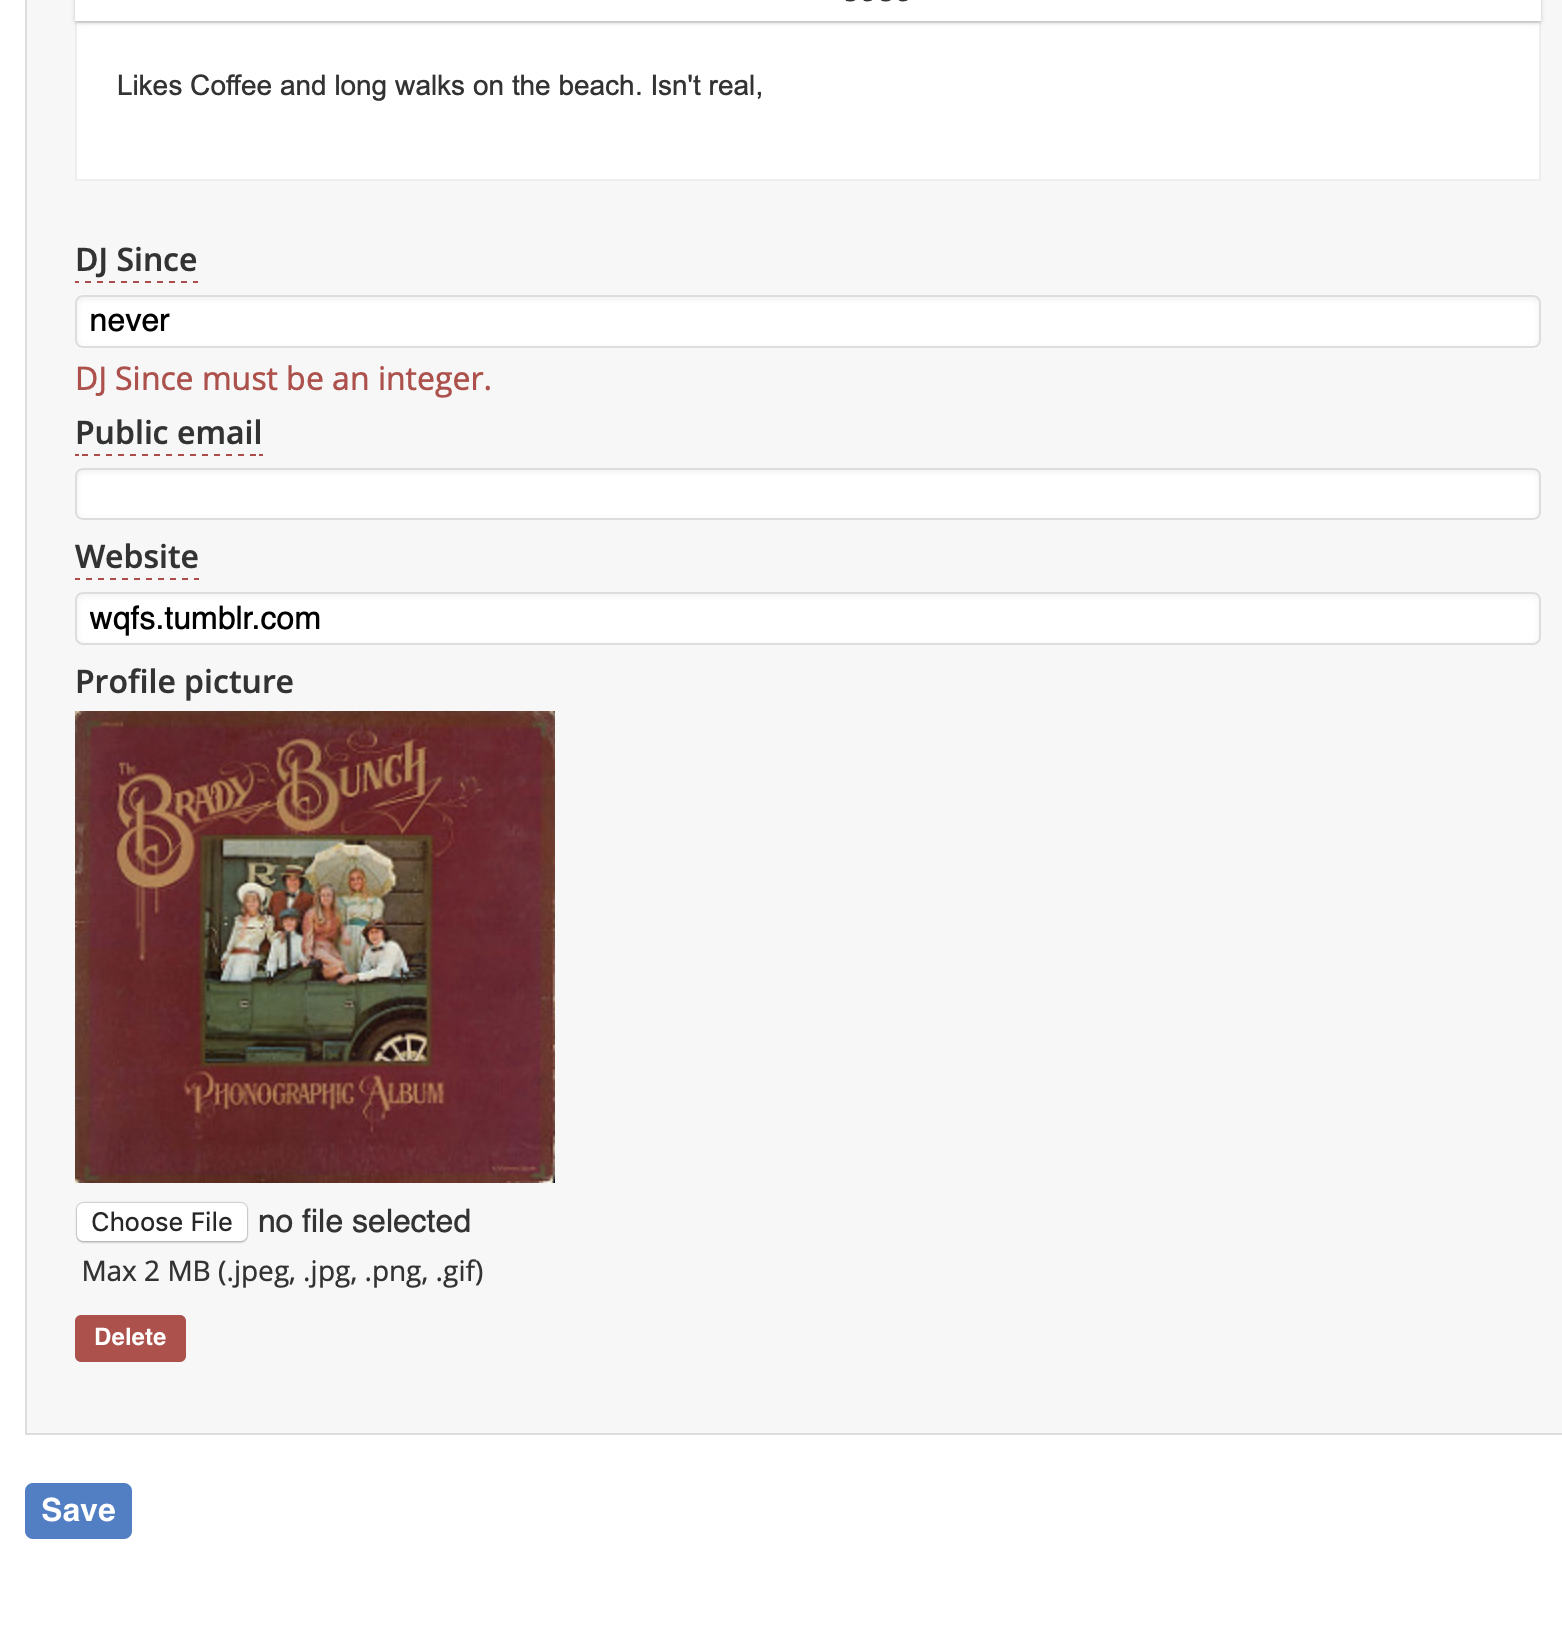
\includegraphics[width=1.0\linewidth, height=5cm]{images/DJ_profile2.png}
%    \label{fig:DJp2}
%    \end{subfigure}
 
 \caption{choosing external of treatg. Recommended that keep the \textbf{three L1, L2  and L3} only in a folder and choose any file from the folder}
\label{fig6}
\end{figure}
    
    
    
    \subsubsection{Day of Run}
    As the name suggests, Day of run denotes the entire process that needs to be run for a particular day. For every day, the process may vary. 
    \begin{enumerate}
        \item L1  Loop1
        \item L2  Loop2
        \item L3  Loop3
        \item D4  In-run stability   
        \item D5  In-run stability
        \item D6  endurance test
    \end{enumerate}
    
    
    
    
    \subsubsection{Analysis type}
    There are two modes of Analysis type namely internal and external.
    \begin{enumerate}
        \item Internal is used for automatic analysis for the acquired data
        \item External is made so that the complete analysis like conformance report can be generated from the Treatg files that have been created earlier.
    \end{enumerate}
   
   \begin{figure}[H]
 
    \begin{subfigure}{1.0\textwidth}
    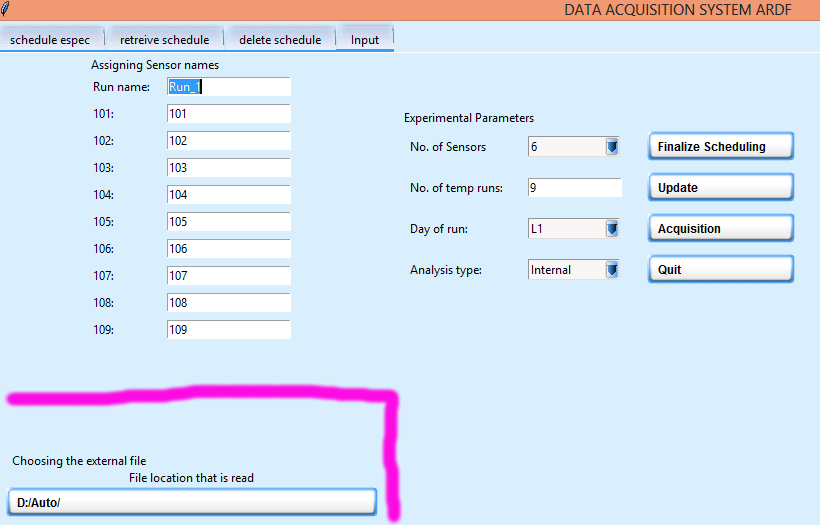
\includegraphics[scale=0.5]{images/choosing_external.png} 
    \label{fig:DJp1}
    \end{subfigure}
%    \begin{subfigure}{0.5\textwidth}
%    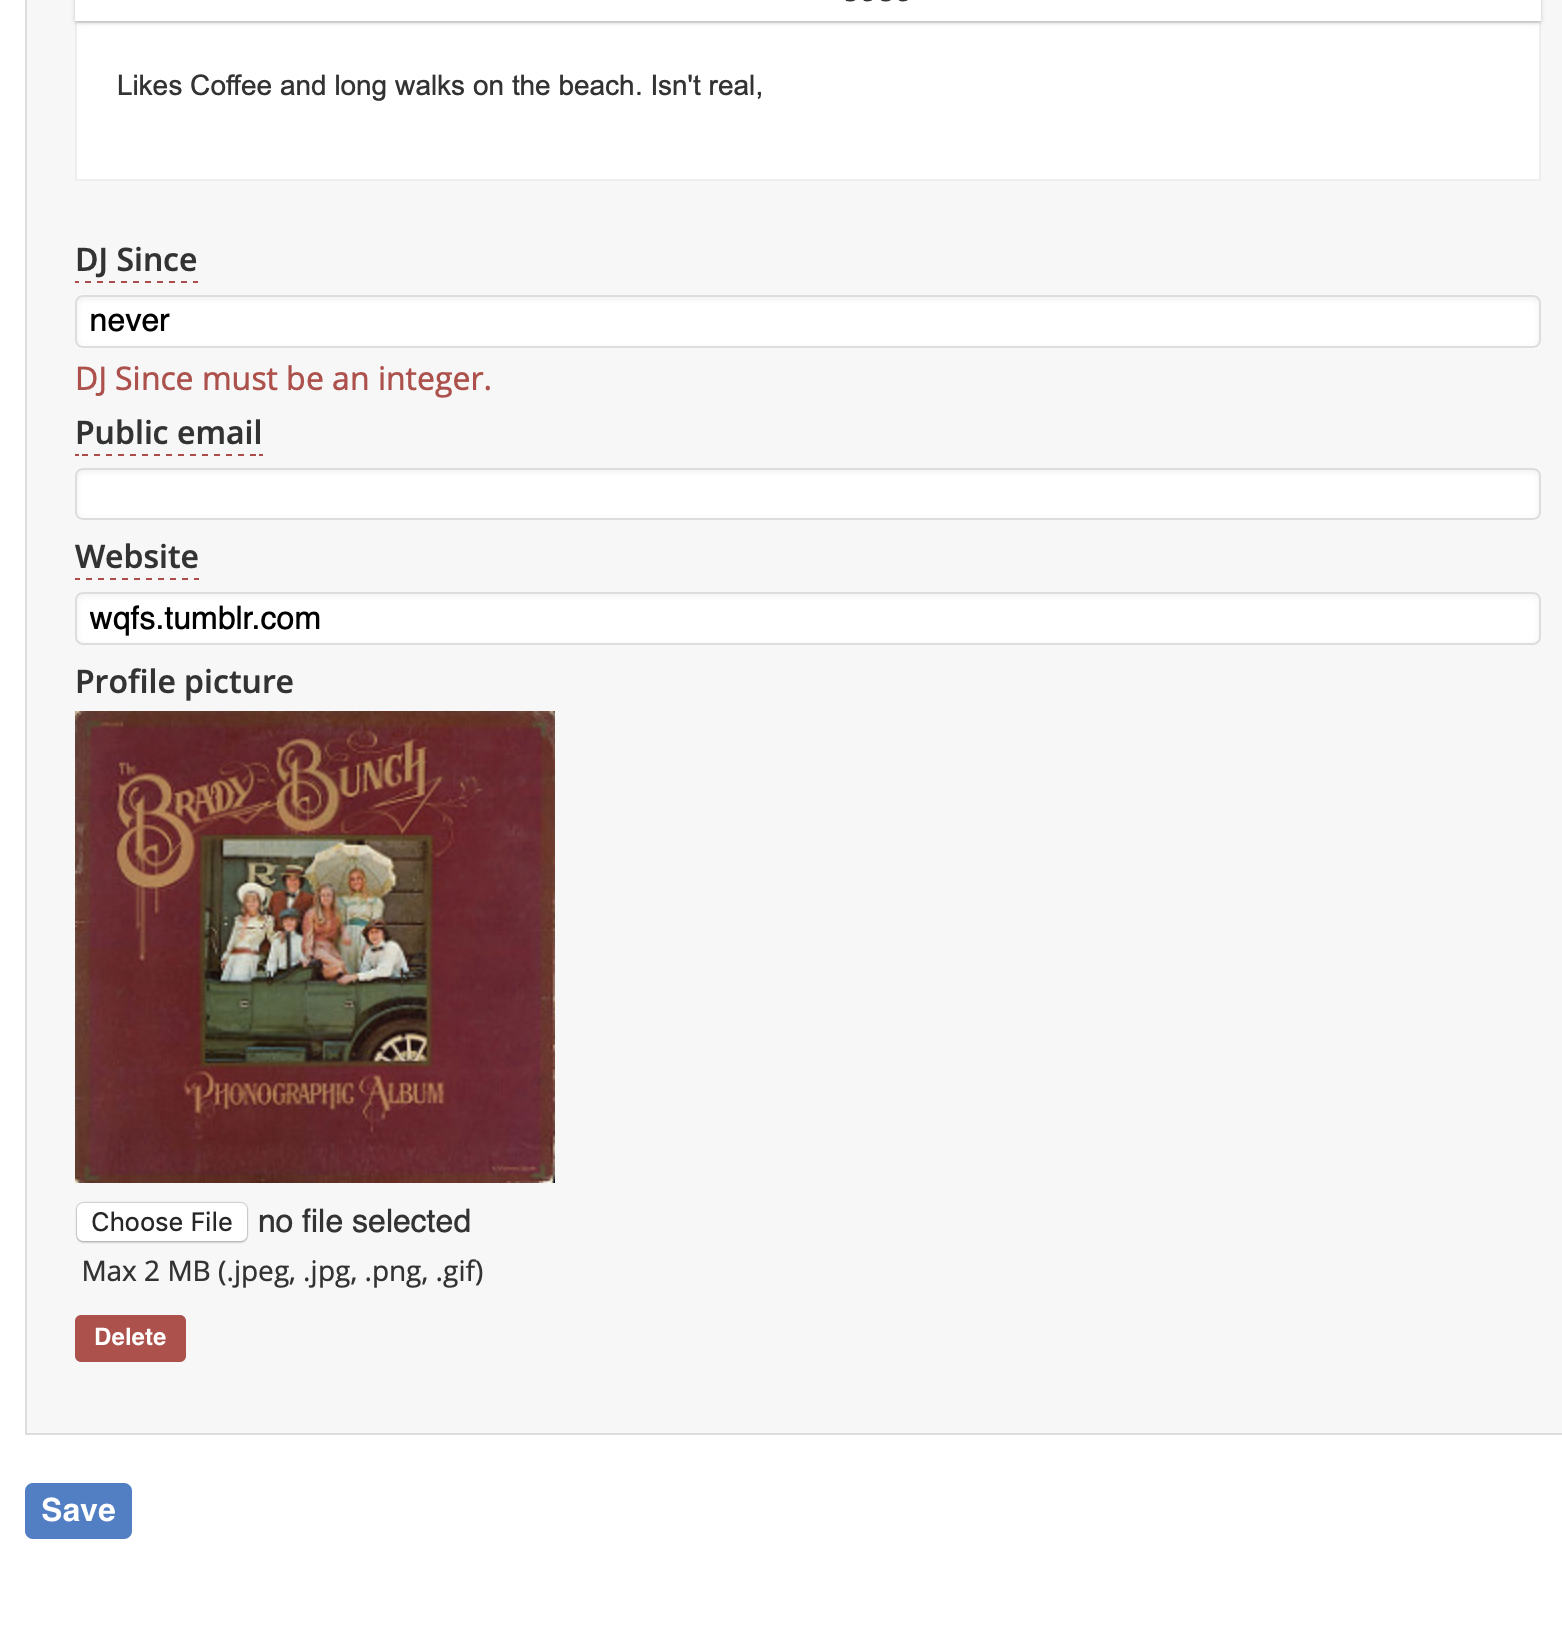
\includegraphics[width=1.0\linewidth, height=5cm]{images/DJ_profile2.png}
%    \label{fig:DJp2}
%    \end{subfigure}
 
 \caption{choosing external of treatg. Recommended that keep the \textbf{three L1, L2  and L3} only in a folder and choose any file from the folder}
\label{fig6}
\end{figure}
   
   
   
   
   
   
   
   
   
    Therefore, whenever \textbf{Analyze} (button) to be used, it is always the internal (default). Only when the occasion arises to use the treatg input files, which are generally made elsewhere. The \textbf{Perform Treatg} (button) may be used 
 
    
 
 
 
    \section{Acquisition}
    
    \subsection{Choose D4 temp}
    In case the chosen day is D4. Care should be taken to choose the desired D4 temperatures. This extra feature has been added as there is a need to run D4 with only a single temperatures. Check boxes have been provided and the desired temperatures needed  to be checked. 
    
    \begin{figure}[H]
 
    \begin{subfigure}{1.0\textwidth}
    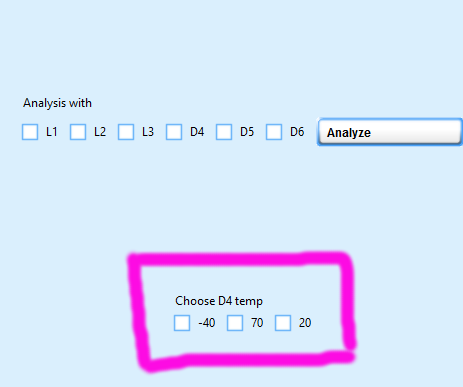
\includegraphics[scale=0.5]{images/choose_D4_temp.png} 
    \label{fig:DJp1}
    \end{subfigure}
%    \begin{subfigure}{0.5\textwidth}
%    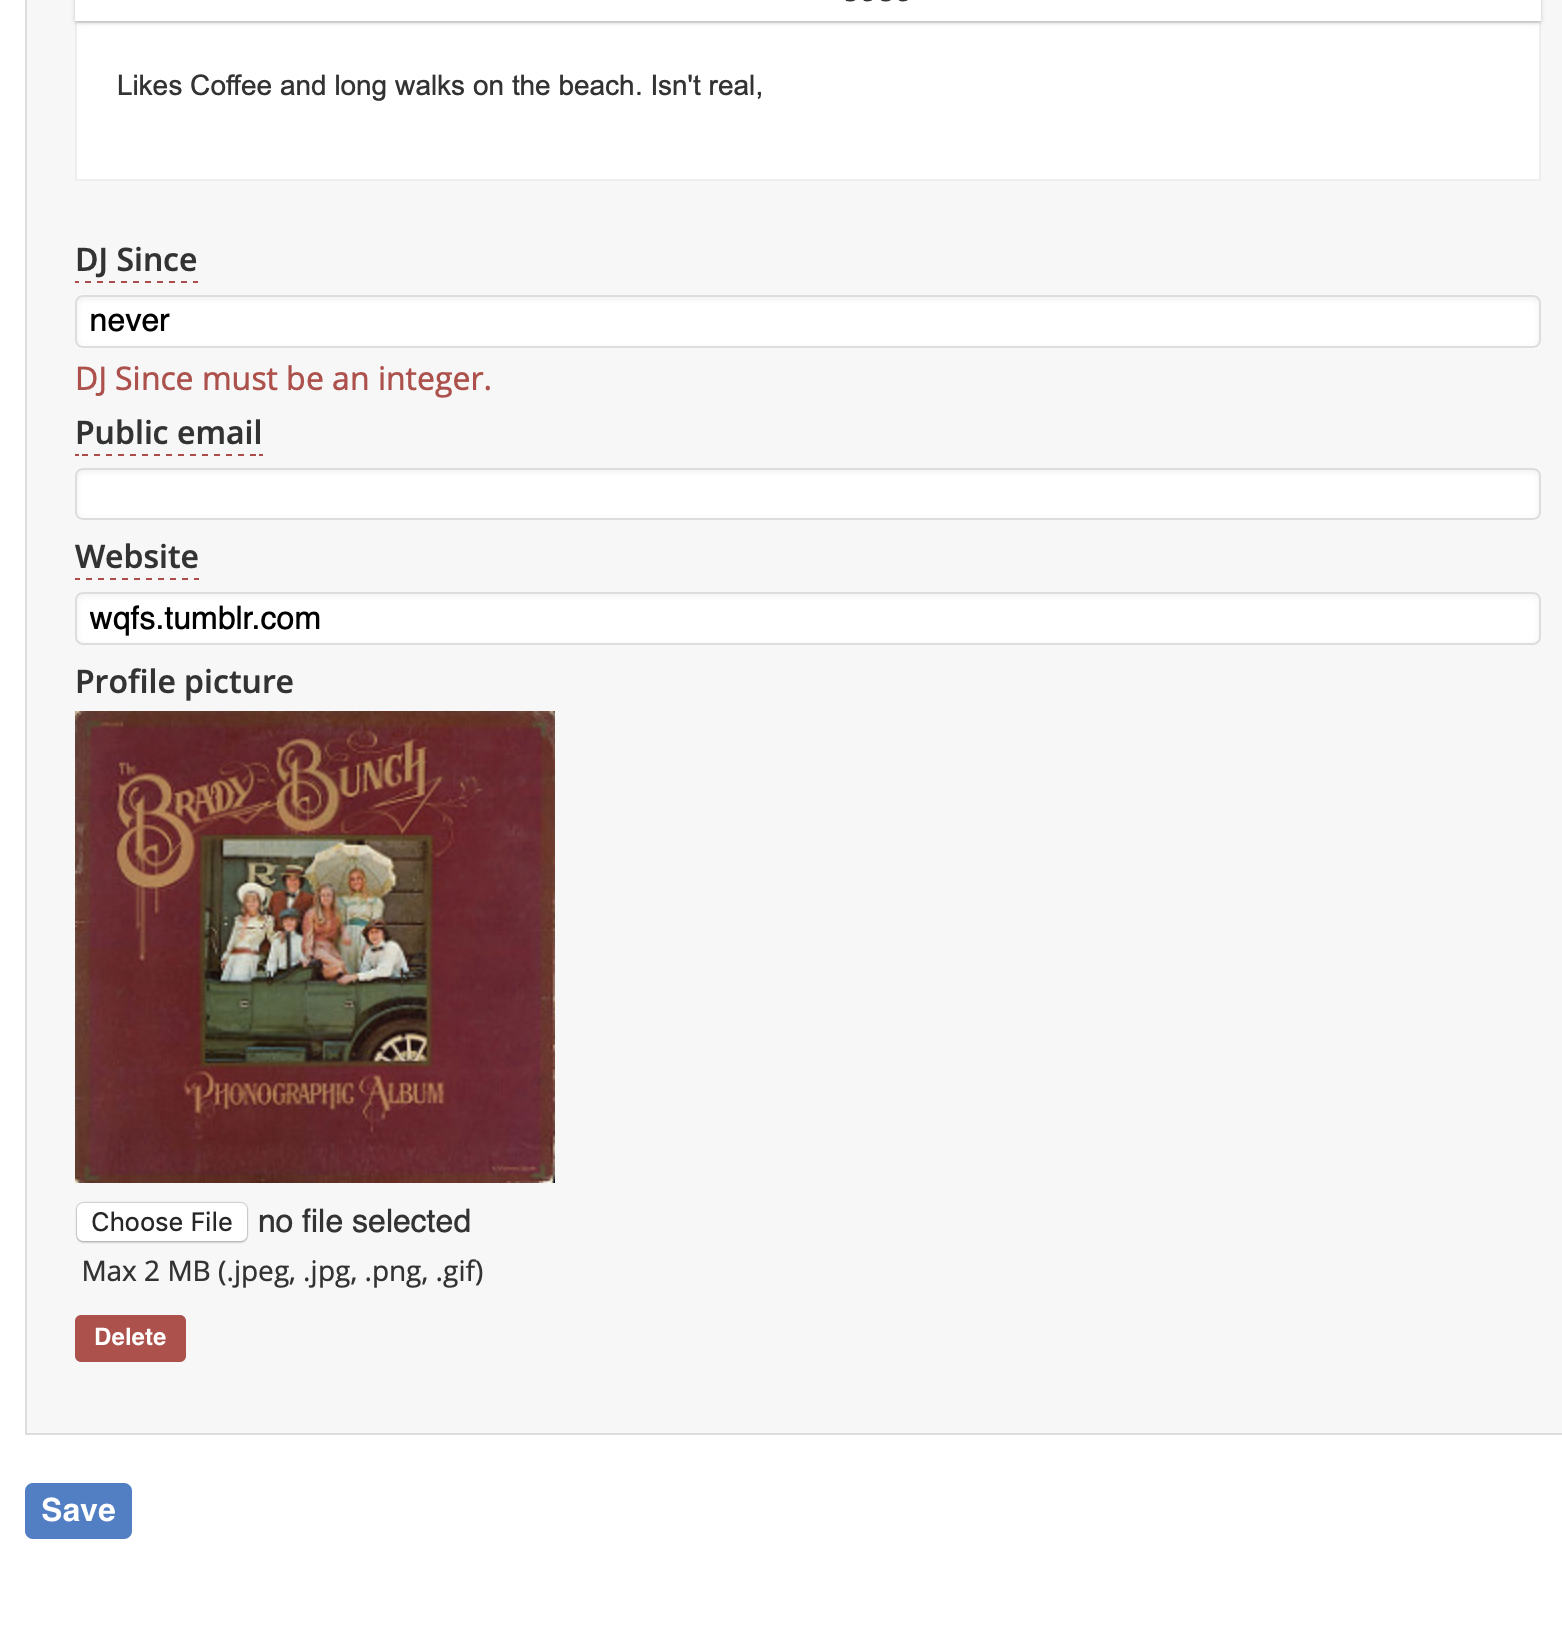
\includegraphics[width=1.0\linewidth, height=5cm]{images/DJ_profile2.png}
%    \label{fig:DJp2}
%    \end{subfigure}
 
 \caption{Choose D4 temp}
\label{fig6}
\end{figure}
    
    \subsection{Update Button}
    This is the button that needs to be pressed before either acquisition or Analysis. After changing the fields (after typing the details) this is the button that needs to be pressed for updating the desired process to the software.
    
    
    
    \subsection{Acquisition Button}
    Since the desired process would have been updated to the software using the Update button. Press the acquisition button to obtain  the acquisition of the desired day. 
   
    
    
     \section{Analysis}
    There are two modes of Analysis type namely internal and external.
    \begin{enumerate}
        \item Internal is used for automatic analysis for the acquired data
        \item External is made so that the complete analysis like conformance report can be generated from the Treatg files that have been created earlier.
    \end{enumerate}
    \subsection{External Analysis}
    
    \begin{itemize}
        \item choose external in type ofanalysis
        \item  Recommended that keep the \textbf{three L1, L2  and L3} only in a folder and choose any file from the folder
        \item   Create a file name with inrun \textunderscore stability.txt in the same folder containing all the three input files of treatg and place the matrix that the conformance report requires in that file
        \item  press \textbf{perform Treatg}
        \item This should generate conformance report from the files.
    \end{itemize}
   
    
   
   \begin{figure}[H]
 
    \begin{subfigure}{1.0\textwidth}
    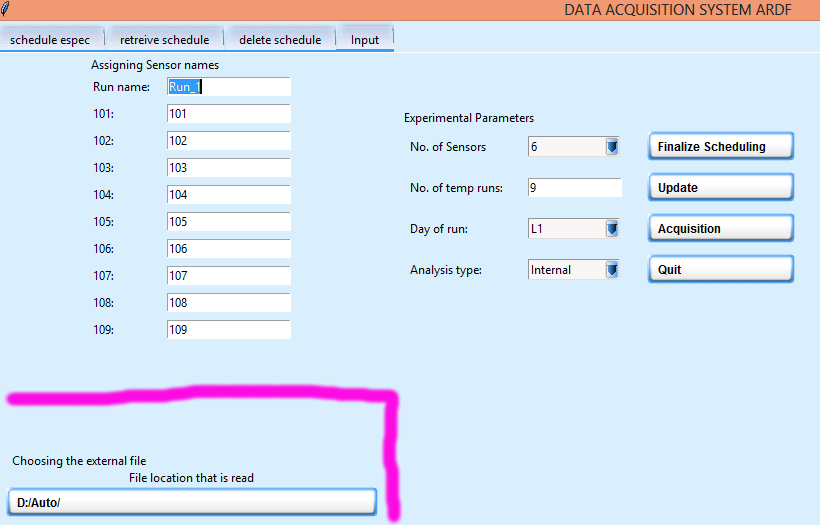
\includegraphics[scale=0.5]{images/choosing_external.png} 
    \label{fig:DJp1}
    \end{subfigure}
%    \begin{subfigure}{0.5\textwidth}
%    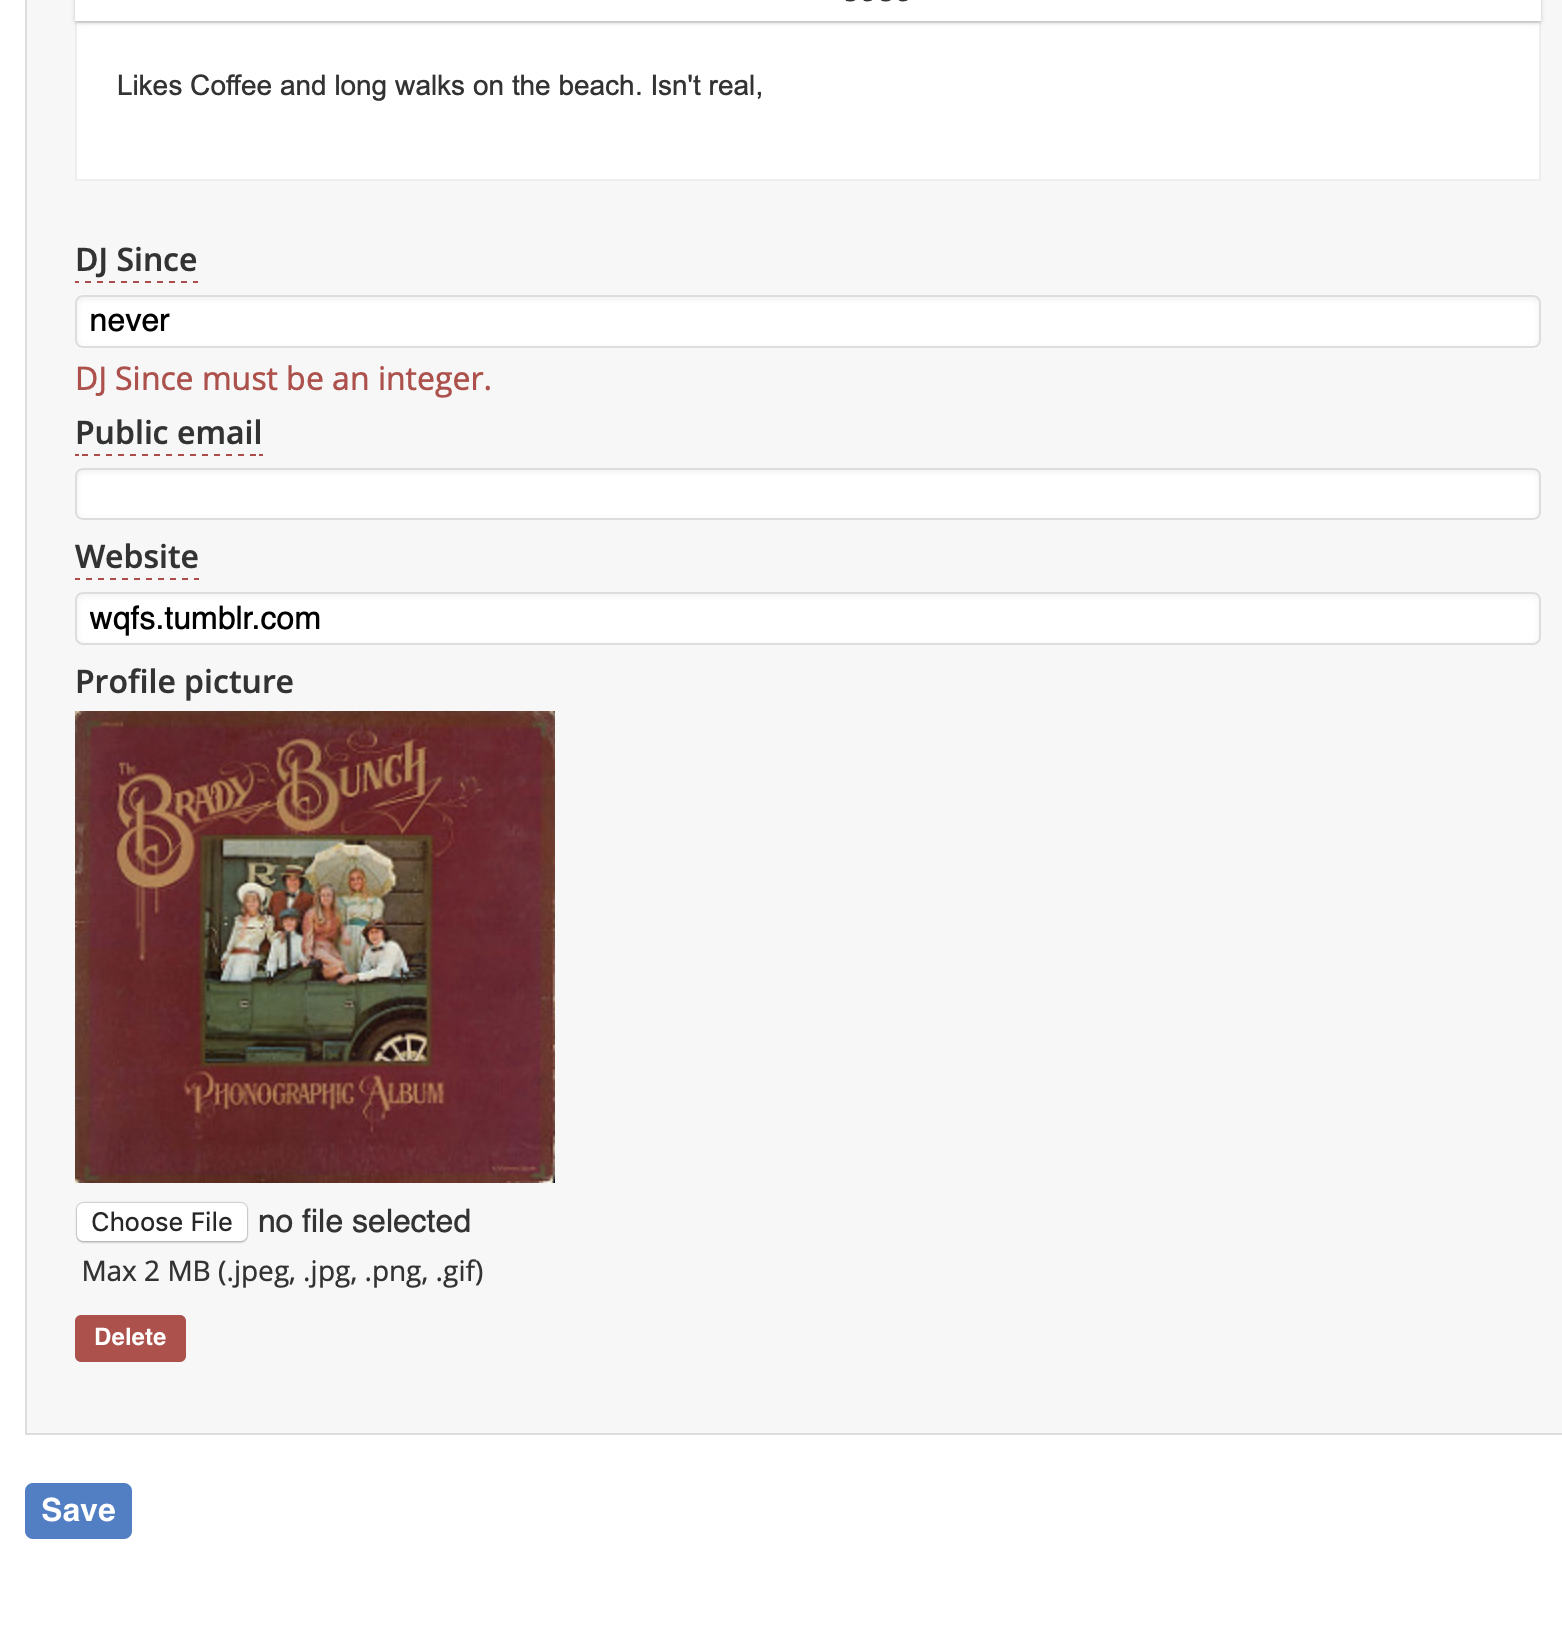
\includegraphics[width=1.0\linewidth, height=5cm]{images/DJ_profile2.png}
%    \label{fig:DJp2}
%    \end{subfigure}
 
 \caption{choosing external of treatg. Recommended that keep the \textbf{three L1, L2  and L3} only in a folder and choose any file from the folder, then choose external type of analysis and press \textbf{perform Treatg} . This should generate conformance report from the files }
\label{fig6}
\end{figure}
   
   
   
  Therefore, whenever \textbf{Analyze} (button) to be used, it is always the internal (default). Only when the occasion arises to use the treatg input files, which are generally made elsewhere. The \textbf{Perform Treatg} (button) may be used 
 
    
    
    
    
    
    
    
    \subsection{ Internal Analysis}
    Special care has been taken to design the analysis part of the program. The requirement goes as the user should be able to run the analysis program even prior to all the days of the acquisition is finished. Thus a resources folder is made at \path{D/Auto/resources/}. This folder contains dummy files. FOr those runs for which all the acquisition  files are not present. These files present in the resources folder gets added. 
    
    
    
    
    
    
    
    
    
    
    
    
    
    
    
    
    
    
    
    
    
    
    
    
    \subsubsection{Run name}
     Please type the same run name with which the data acquisition has been performed. 
    
    \subsubsection{Choose D4 temp}
    In case the  D4 is ticked,  Care should be taken to choose the desired D4 temperatures. Please check those temperatures with which acquisition took place.
    
     \begin{figure}[H]
 
    \begin{subfigure}{1.0\textwidth}
    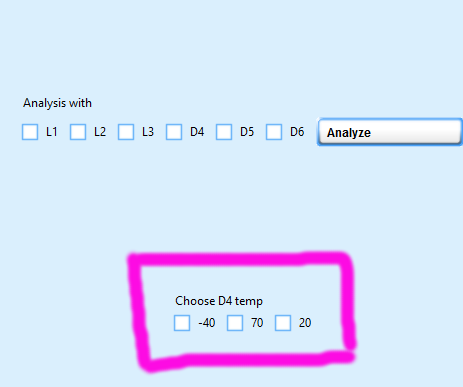
\includegraphics[scale=0.5]{images/choose_D4_temp.png} 
    \label{fig:DJp1}
    \end{subfigure}
%    \begin{subfigure}{0.5\textwidth}
%    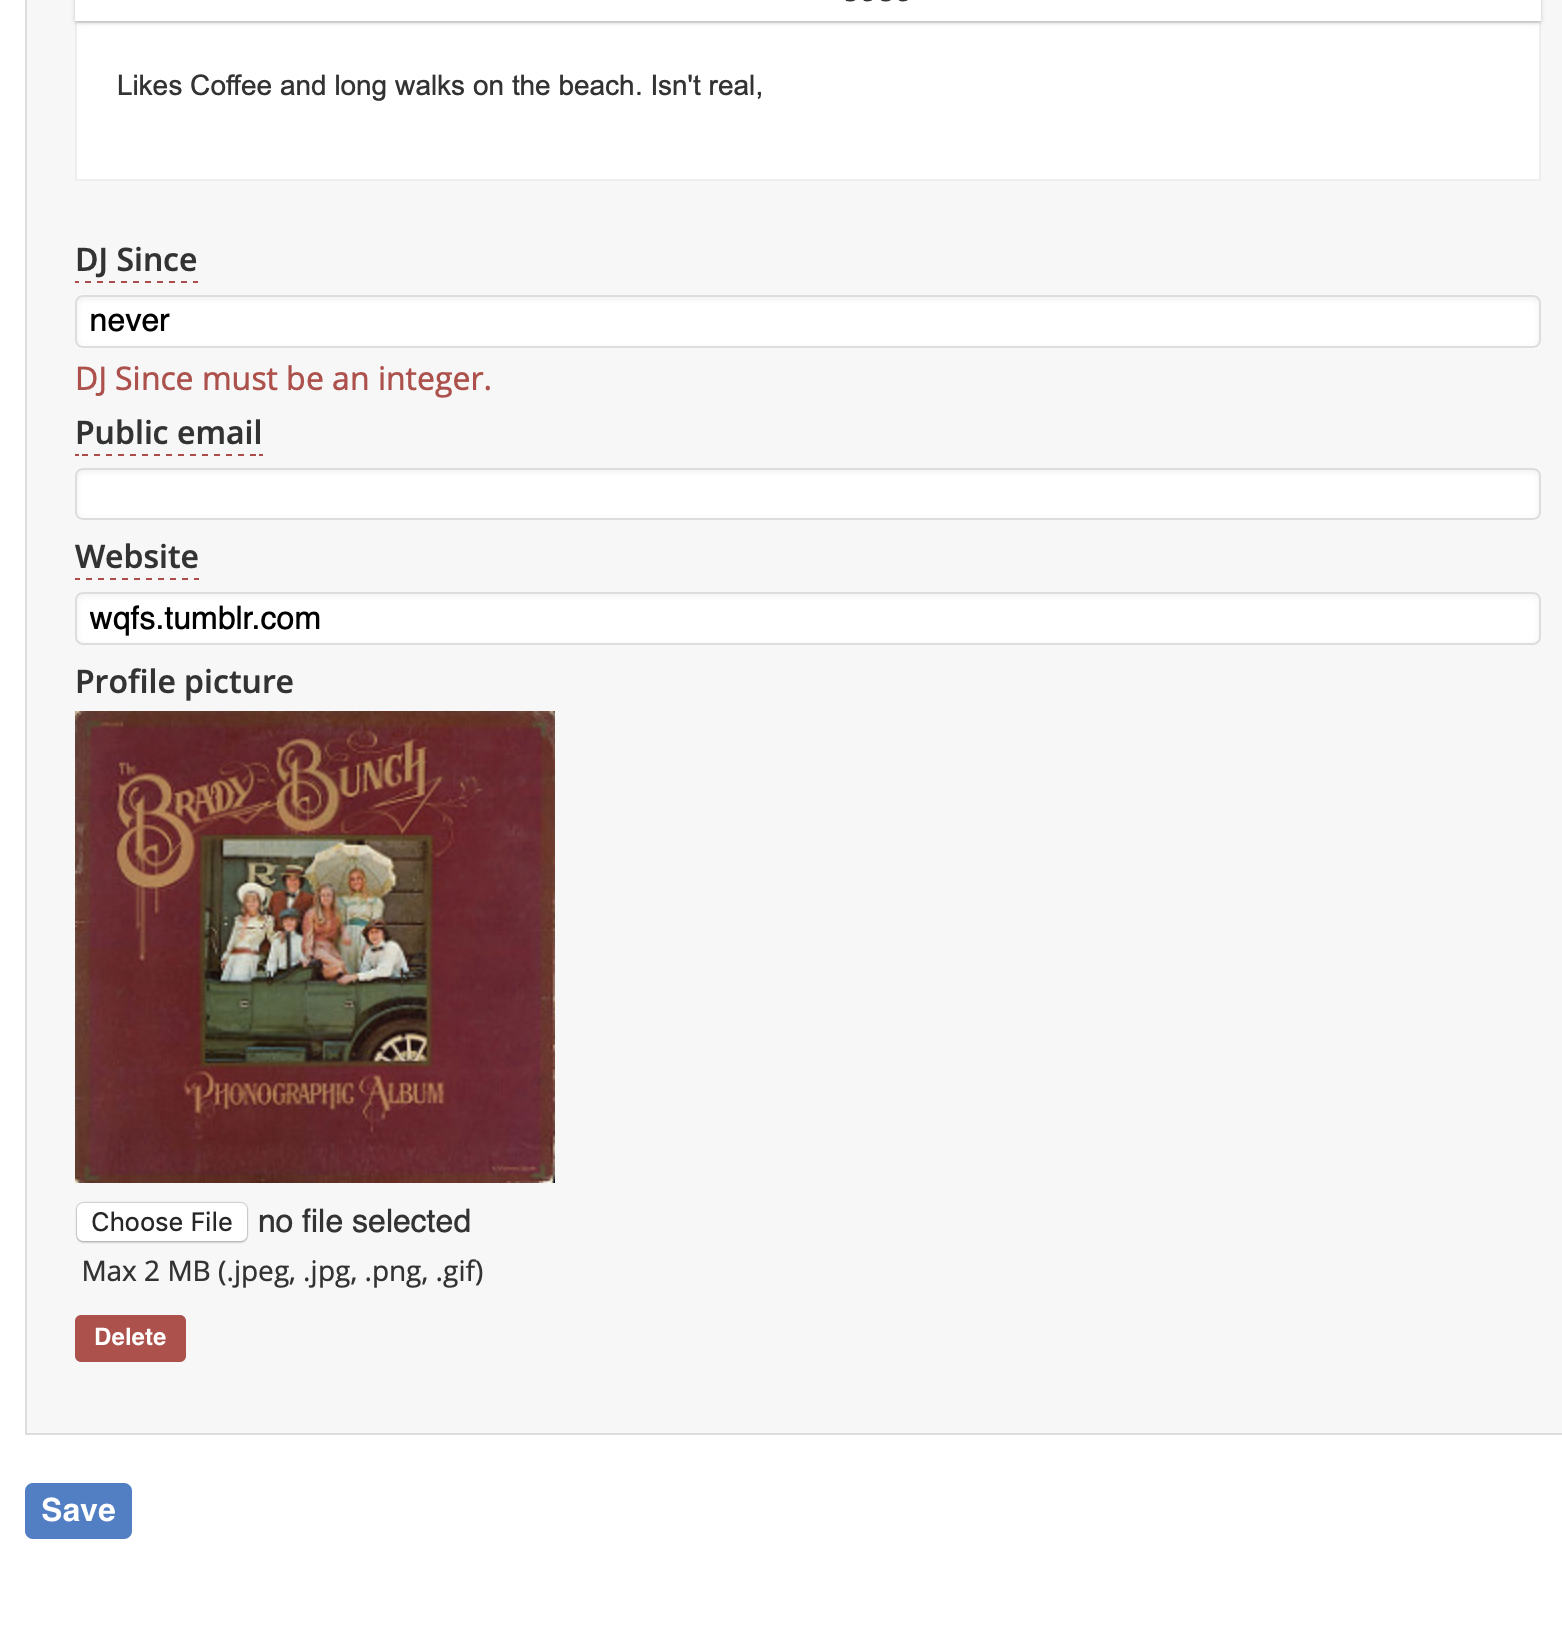
\includegraphics[width=1.0\linewidth, height=5cm]{images/DJ_profile2.png}
%    \label{fig:DJp2}
%    \end{subfigure}
 
 \caption{Choose D4 temp}
\label{fig6}
\end{figure}
     
    
    
    
    \subsubsection{Tick the check boxes for which acquisition happened }
    When the user ticks the days the acquisition has happened, the software understands and obtains the dummy acquisition data from the resources folder for those days acquisition data is not present. 
    \begin{figure}[H]
 
    \begin{subfigure}{1.0\textwidth}
    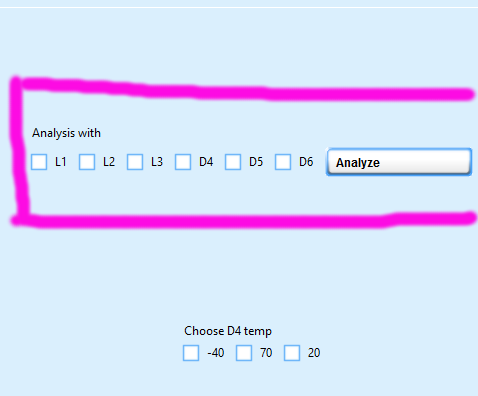
\includegraphics[scale=0.5]{images/Analysis.png} 
    \label{fig:DJp1}
    \end{subfigure}
%    \begin{subfigure}{0.5\textwidth}
%    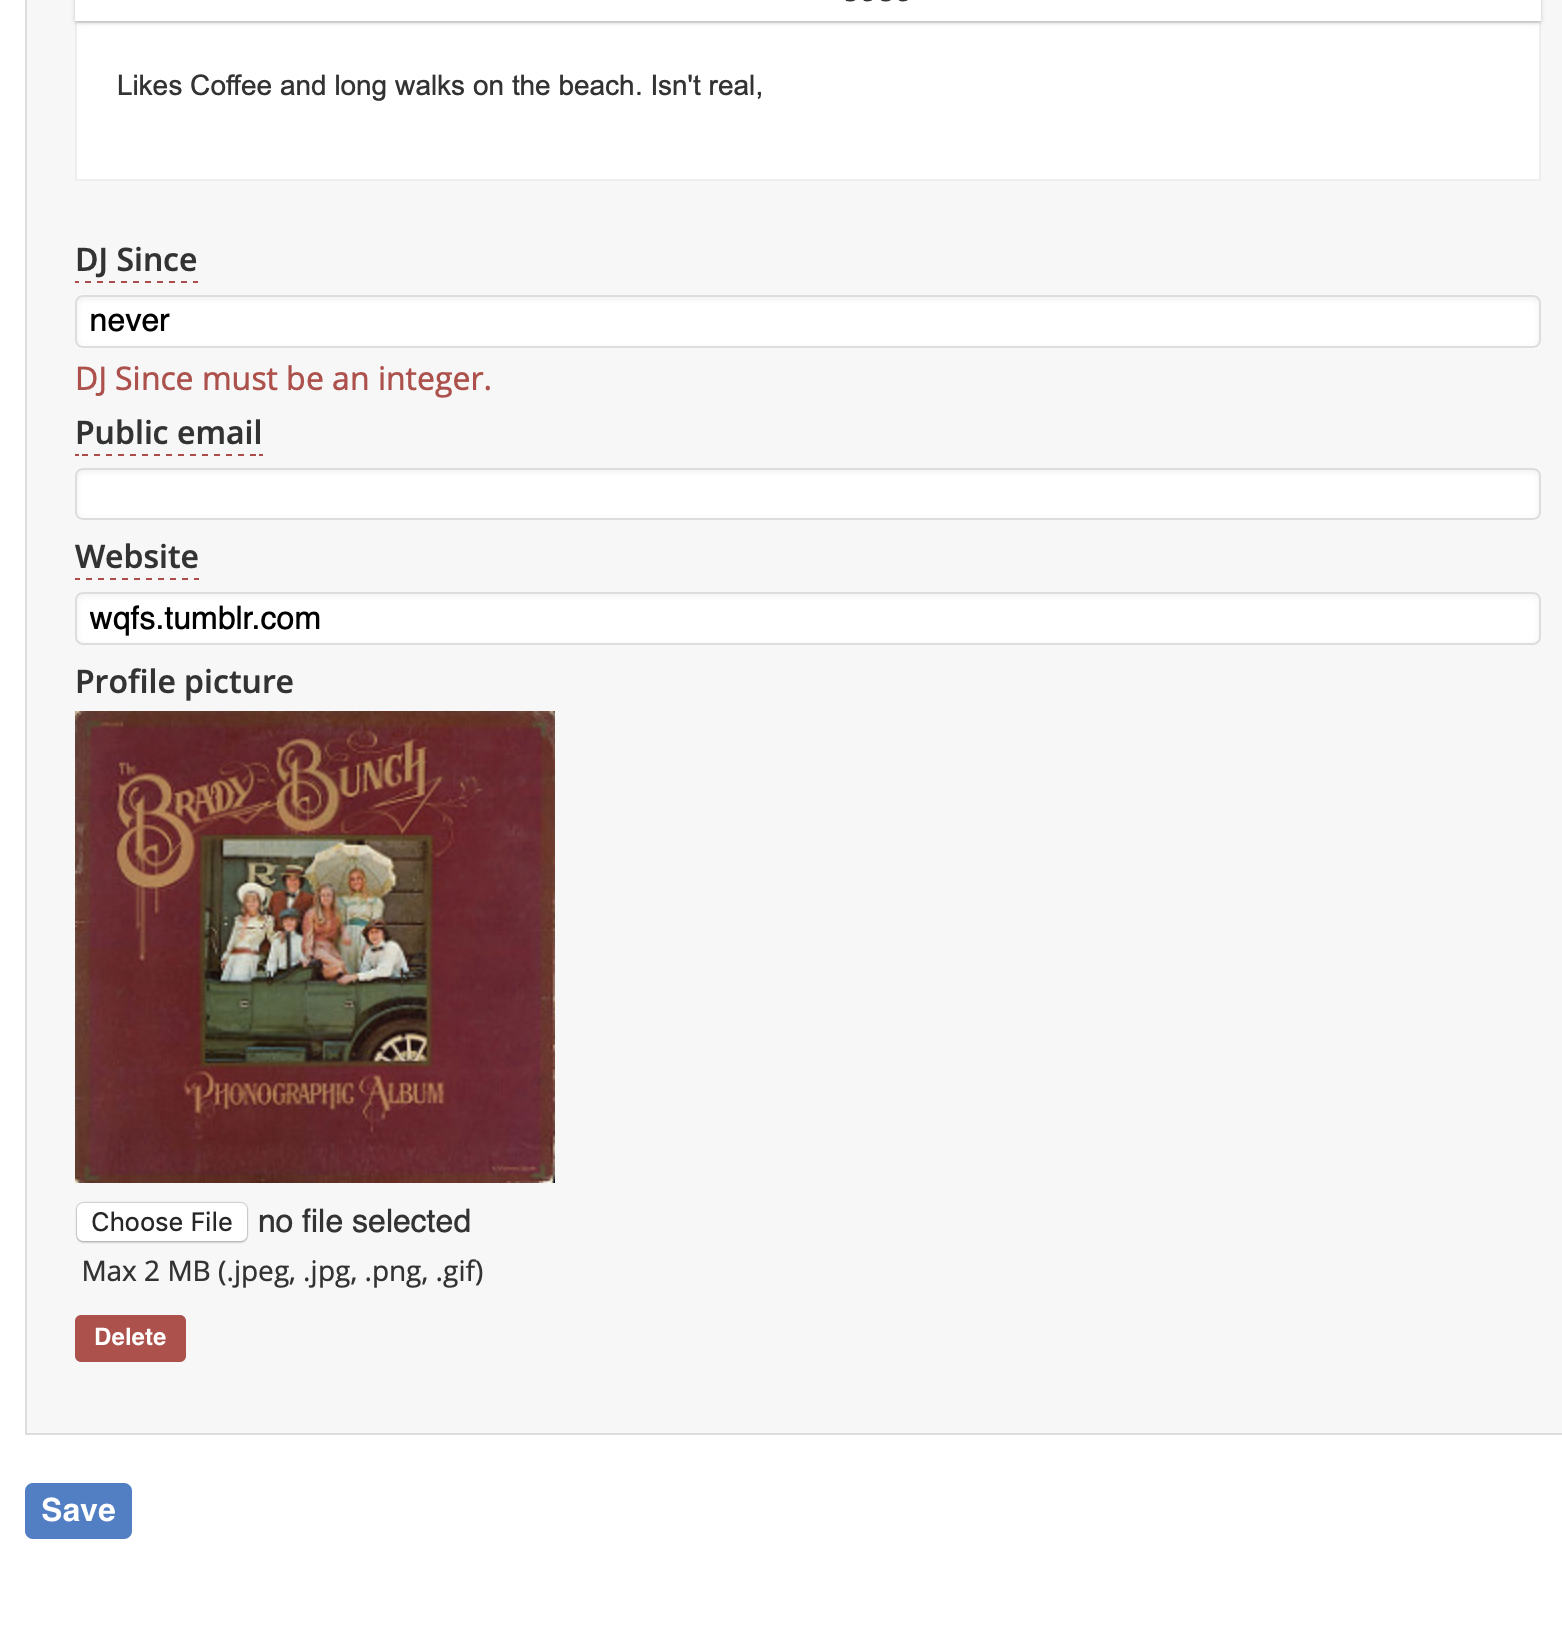
\includegraphics[width=1.0\linewidth, height=5cm]{images/DJ_profile2.png}
%    \label{fig:DJp2}
%    \end{subfigure}
 
 \caption{Shown are different check boxes. Please check the boxes for those days acquisition has happened. Then in case D4 is present check the temperatures and press analyze}
\label{fig6}
\end{figure}
    
    
    
    
    \subsubsection{Update Button}
    This is the button that needs to be pressed before either acquisition or Analysis. After changing the fields (after typing the details) this is the button that needs to be pressed for updating the desired process to the software.
    
     \subsubsection{Press Analyze button}
    Please press analyze button. Then, the   following files are created, with the described work flow:
    
    \begin{enumerate}
        \item  First the software verifies whether all the information of those days are present as the user claims. For example, user ticks L2, it checks the data is present for L2.
        \item Then it adds the dummy data from  \path{D/Auto/resources/} for the other days for which the acquisition has still yet to happen. 
        \item Then combining all the data i.e user obtained data and dummy data, the acquisition takes place. This feature is added so that the user can verify his results instantly.  
        
    \end{enumerate} 
    
     
    
    
    
    \subsubsection{Output}
    Please wait for 5 minutes, during this time the software generates all the desired output files. The output files that the software generates is enumerated below:
    
    \begin{enumerate}
        \item First it divides the data into corresponding channels (by default 6).
        \item Placing the data into folders with the name of the folder  as the sensor name
        \item Then creating input files for the Treatg software in a specific format
        \item Automatically running Treatg software for each of these channels 
        \item Analyzing the obtained output from the Treatg Russian software and calculating the parameters for the conformance report
        \item Obtain the In-run stability matrix and calculating the parameters for the conformance report
        \item Generating graphs in png from the ouput of the Treatg software
        \item Generating the Origin file for obtaining the desired graphs in the origin .opj format
        \item Generating the excel files from the D4 and D5 runs and making excel macros
        \item Generating the conformance report
        \item Generating the Endurance report
    \end{enumerate}
    
In short open the spyder, press play button. Then,affter connecting GUI appears. Select the day that needs to be run and press acquisition or analyze button. In short that is all that is needed to be done torun the program. However, many other features have been added and explained to ease the user experience and save time of acquiring data and analyzing to obtain an half a dozen files.

\newpage

\listoffigures

\end{document}
